\nonstopmode

\documentclass
[
    a4paper,
    twoside,
    12pt,
]
{report}
\usepackage[utf8]{inputenc}
\renewcommand{\familydefault}{\rmdefault}
\usepackage[a4paper, left=3.19cm, right=3.19cm, top=2.54cm, bottom=2.54cm]{geometry}
\usepackage[american]{babel}
\usepackage{csquotes}
\usepackage{float}
\usepackage{enumerate}
\usepackage[bottom]{footmisc}
\usepackage{array}
\usepackage{ntheorem}
\usepackage{parskip}
\usepackage[right]{eurosym}
\usepackage{xcolor}
\usepackage[hyphens]{url}
\usepackage{makeidx}
\usepackage{multicol}
\usepackage{theorem}
\usepackage{amsmath}
\DeclareMathOperator*{\argmax}{arg\,max}
\usepackage{listings}
\usepackage{graphicx}
\usepackage{subcaption}
\usepackage{pgfplots}
\pgfplotsset{compat=1.5}
\usepackage{csvsimple}
\usepackage{fancyhdr}
\usepackage{colortbl}
\usepackage{bchart}
\usepackage[hidelinks]{hyperref}
\usepackage{setspace}
\usepackage{mathptmx}
%\usepackage{showframe}
\pagestyle{plain}
\rhead{\thepage}
\sloppy

\usepackage[
backend=biber,
style=apa,
citestyle=authoryear
]{biblatex}

\addbibresource{references.bib}
\DeclareLanguageMapping{american}{american-apa}
\def\sectionautorefname{Section}

%\setlength{\unitlength}{1cm}
%\setlength{\oddsidemargin}{0.3cm}
%\setlength{\evensidemargin}{0.3cm}
%\setlength{\textwidth}{15.5cm}
%\setlength{\topmargin}{-1.2cm}
%\setlength{\textheight}{24.7cm}
%\columnsep 0.5cm

%\title{Seminararbeit}
\selectcolormodel{cmyk}{

\newcommand{\Arbeitstitel}
	{
  	Success factors of video game consoles
	}
\newcommand{\Autor}
	{
		Dipl.-Ing. (FH) Lars Bartschat
	}

\newcommand{\MatrikelNr}
	{
		WBPA140000250
	}

\newcommand{\EmailAdresse}
	{
		bartschat@mailbox.org
	}
\newcommand{\Arbeitsart}
	{
		Seminar Paper
	}
\newcommand{\Studiengang}
	{
		Marketing Executive Program
	}
\newcommand{\Hochschule}
	{
		University of Münster
	}
\newcommand{\Lehrstuhl}
	{
		Department of Marketing and Media Research
	}
\newcommand{\Themensteller}
	{
		Prof. Dr. T. Hennig-Thurau
	}
\newcommand{\Betreuer}
	{
		M. Sc. R. Behrens
	}
\newcommand{\Ausgabedatum}
	{
		17.10.2016
	}
\newcommand{\Abgabedatum}
	{
		28.11.2016
	}
\newcommand{\Ort}
	{
		Münster}
			
		
\newcommand{\link}[1]{\ref{#1} (S. \pageref{#1})}
\begin{document}

\begin{titlepage}
    \vspace*{1.0cm}
    \begin{center}
        \begin{Large}
        \textbf{An investigation of accent conversion for non-native and native varieties of English} \\
        \end{Large}
        \vspace*{1.0cm}
        \textit{Kenny W. Lino} \\
        \vspace*{1.5cm}
        M.Sc. Dissertation \\
        \vspace*{0.5cm}
        \begin{figure}[H]
        \centering
        
\includegraphics[scale=0.15]{img/UM-coat-of-arms.png}
    	\end{figure}
       \vspace*{1.0cm}
       Department of Intelligent Computer Systems \\
       Faculty of Information and Communication Technology \\
       University of Malta \\
       2019 \\
       
       \vspace*{2.0cm}
	   Supervisors: \\
       Claudia Borg, Department of Artificial Intelligence, University of Malta \\
       Andrea DeMarco, Institute of Space Sciences and Astronomy, University of Malta \\
       Eva Navas, Department of Communications Engineering, University of the Basque Country \\
       
       \vspace*{4.0cm}
       Submitted in partial fulfilment of the requirements for the Degree of \\
       European Master of Science in Human Language Science and Technology
    \end{center}



\end{titlepage}

\onehalfspacing
\pagenumbering{Roman}

\cleardoublepage

\begin{center}
  M.Sc (HLST) \\
  \uppercase{\textbf{Faculty of Information and \\
  Communication Technology \\ University of Malta \\ }}
  \vspace*{0.5cm}
  Declaration \\
\end{center}
  \vspace*{1.5cm}
        Plagiarism is defined as ``the unacknowledged use, as one's own work, of work of another person, whether or not such work has been published" (Regulations Governing Conduct at Examinations, 1997, Regulation 1 (viii), University of Malta). \\

I, the undersigned, declare that the Master's dissertation submitted is my own work, except where acknowledged and referenced. \\

I understand that the penalties for making a false declaration may include, but are not limited to, loss of marks; cancellation of examination results; enforced suspension of studies; or expulsion from the degree programme. \\
       
       \vspace*{1.5cm}
	     Student Name: Kenny W. Lino \\
       Course Code: CSA5310 HLST Dissertation \\
       Title of work: An investigation of accent conversion for non-native and native varieties of English\

       \vspace*{1.0cm}
       Signature of Student: \\

       \vspace*{1.0cm}
       Date: January 7, 2019

\newpage
\section*{Acknowledgments}

I would first like to thank my gracious advisors at the University of
Malta, Claudia Borg and Andrea DeMarco for being supportive and
extremely understanding. Without their input and encouragement, I would
not have been able to complete this work.

I would also like to give thanks to the LCT programme for allowing me to
partake in such a life-changing experience where I was able to study and
learn about life in places I could only dream about. Thanks to the
programme, I was able to find a new outlet for my passion in language
and linguistics and make life-long friends. I will never forget this
experience.

\newpage
\section*{Abstract}
\addcontentsline{toc}{section}{Abstract}

Accent conversion (AC), the process of transforming the accent of one
speaker as if they had the accent of another speaker, has been cited as
a prospective solution for challenges faced in language learning and
voice-based technologies. Works such as \textcite{aryal2014, zhao2018a}
have found some success in using accent conversion to minimize the
accents of various non-native speakers, while work such as
\textcite{mohammadi2017} points to the multiple applications of voice
conversion as a whole. Despite these works, accent conversion still
remains a relatively new section of research, with plenty to be
investigated.

In this master's thesis, we detail previous research as related to
accents by outlining important theories from the perspective of
linguistics and provide details on how accent conversion arose as a
prospective solution for language learning and voice-based technologies
by discussing research in computer-assisted pronunciation training and
automatic speech recognition systems. We then detail our experiments
with accent conversion using a traditional Gaussian Mixture Model
approach following \textcite{aryal2014} using the ARCTIC/L2-ARCTIC
corpora to test non-native to native conversion, and the Accents of the
British Isles (ABI) corpus to test conversion between two native, but
distinct accents. We compare the performance of accent conversion
between these two separate corpora by recruiting the help of outside
evaluators to do a perceptual study. Through the perceptual study, we
observe that the evaluators agree that the converted audios in both
corpora have the desired accent; however there are issues in maintaining
the identity of the speakers. We conclude with discussion on possible
sources for the results and directions for future work.
\cleardoublepage
\tableofcontents
\addcontentsline{toc}{section}{Contents}
\clearpage
\listoffigures
\addcontentsline{toc}{section}{List of Figures}

\cleardoublepage
\section*{List of Abbreviations}
\addcontentsline{toc}{section}{List of Abbreviations}
\begin{tabular}{ll}
    ABI   & Accents of the British Isles Corpus \\
    AC    & Accent conversion \\
    CAPT    & Computer Assisted Pronunciation Training \\
    CP      & Critical Period \\
    GMM     & Gaussian Mixture Model \\
    L1/L2    & First and second language \\
    LSTM & Long-short term memory \\
    MFCC & Mel-frequency cepstrum coefficient \\ 
    TTS   & Text-to-speech \\
    VC   & Voice conversion \\
    
\end{tabular}

\clearpage
\cleardoublepage
\pagenumbering{arabic}
\setcounter{page}{1}

\chapter{Introduction}

\hypertarget{what-is-an-accent}{%
\section{What is an ``accent''?}\label{what-is-an-accent}}

Before continuing on, it is best to define what accent is, especially in
the context of this work. The definition of `accent', much like any
other word can fluctuate based on the context it is used in, and by whom
the word is used. Fundamentally, accents consist of a number of
features, including the vowels and consonants, the stress, rhythm,
intonation, and even pauses that a speaker uses. The variation in these
features contribute to what many known as \emph{accent}, or variations
in pronunciation across speakers based on location, ethnicities, social
classes, native languages, etc \parencite{crystal2008}. Accents can be
considered to be a part of dialects, where users of the same language
may have variations beyond pronunciation, such as usage in vocabulary or
grammar. The line between accents and dialects may often be blurred in
everyday discussions and even in academic analyses as accent and dialect
(as well as language) could be considered to be on a continuum, but for
the sake of simplicity, we consider `accent' to be solely variations in
pronunciation in this work.

\hypertarget{motivation-for-this-work}{%
\section{Motivation for this work}\label{motivation-for-this-work}}

Technology has flourished and led to a number of new state-of-the-art
systems such as improvements in commercial speech recognition and
machine translation. However, it can be argued that these benefits have
not reached all potential users and uses to the same extent. For
example, many commercial systems like Google Translate, Siri, Alexa,
etc. have grown in the number of languages they have available, but when
considering the robustness of these systems across languages, it is
often evident that the systems function much better with languages that
have more speakers across the globe such as English or Spanish. In some
cases such as with newer products, a user's native language might not
yet even be available, which can cause them to relegate to English.

These systems are also often better equipped to work with specific
language varieties, which are often considered to be the `standard' or
more common variety of that language. In the context of speech
recognition systems, this means that this could cause potential
challenges for speakers of other varieties-- or \emph{accents}, whether
it be another native but `non-standard' accent or a non-native accent.
This issue can be observed in various viral videos, such as an Italian
grandmother who is trying to activate a Google Home device by saying,
``Okay Google!'' \parencite{actis2017} or another video where a woman is
trying to get her Amazon Alexa device to play a song called
``Something's Cooking in My Kitchen by Dana'' \parencite{newsflare2018}.
In both cases, both women have issues with their devices properly
understanding them likely because they speak English with an accent that
the systems are not (well-)trained on.

Yet when it comes to accents, teaching them can be as equally difficult
as trying to have them recognized by speech recognition systems. This
extends into language teaching and learning as well, where learners of a
second language often have trouble acquiring proper pronunciation. In
fact, pronunciation has been a large standing challenge in language
learning due to its complex nature as observed in second language
learning research \parencite{lenneberg1967a, scovel1988a, flege1995}.
Unlike grammar and vocabulary, which many language learners acquire
without issue, pronunciation can be challenging to both learn and teach
due to the lack of clarity on how to teach it \parencite{darcy2012}.
This is because pronunciation involves a number of nuanced
characteristics, including stress, rhythm, vowels, and consonants, which
can vary just small enough for one language or accent to draw a
distinction, while others conflate them.

In order to address these issues in speech recognition and language
learning, researchers have investigated variation solutions. Linguists
focused on language learning and phonetics have examined the underlying
causes of what creates obstacles in learning an accent, with some
concluding that native-like accents are nearly unobtainable after a
certain age threshold. Regardless of this conclusion, some researchers
have turned to language technology to develop potential pronunciation
training systems with the hopes of any possible accent reduction.
Earlier studies using some of these pronunciation training systems have
shown that while they have the potential, many of them suffer from the
lack of appropriate feedback that the user can understand. Thus, some
researchers have pointed to the potential use of accent conversion as a
mode of feedback as it has been hypothesized that hearing one's voice
pronounce something with the desired accent is better feedback as
compared to a point-based system or spectrograms, which require
specialized training to interpret.

Accent conversion has also been proposed as a potential solution to
challenges in speech recognition. Because speech recognition is often
trained on large amounts of speech data, it can be unrealistic to
attempt to collect sufficient speech data for the endless possible
varieties or accents that exist for a single language. Instead,
researchers have pointed to accent conversion as a possible way to adapt
current available systems to more speakers, with the idea that accent
conversion could change the accent of a speaker into sounding more like
an accent the speech recognition system can better recognize without
training it on a large amount of data. Similarly, accent conversion can
be applied to expand the number of available accents for text-to-speech
systems for languages that may have a large number of accents such as
English or Spanish. This adaptation process can be viewed similarly to
other natural language processing tasks, such as text classification or
part-of-speech tagging of varying genres such as formal news text
vs.~informal blogs or tweets, where currently available systems have
been adapted to perform better on more genres instead of creating
specialized systems for each genre type.

\hypertarget{research-questions}{%
\section{Research Questions}\label{research-questions}}

In this thesis, we focus on investigating the following questions:

\begin{itemize}
\item
  How effective is accent conversion in changing the accent of a
  \emph{non-native speaker} into sounding more like a \emph{native
  speaker} while retaining their voice characteristics, or
  \emph{identity}? Concretely, how effectively can we convert the
  accents of learners of English to sound more like US English while
  retaining their identities?
\item
  How effective is accent conversion to change the accent of two
  \emph{native speakers} of English who speak two \emph{distinct}
  varieties? Specifically, how effectively can we convert the accents of
  speakers of `non-standard' English such as speakers from Scotland, to
  sound more like Standard Southern English while retaining their
  identities?
\item
  Does the same methodology of accent conversion which is most often
  applied to the conversion of non-native to native accents work
  similarly for native to native accent conversion? Concretely, would we
  observe similar performance between non-native to native accent
  conversion vs.~native to native accent conversion?
\end{itemize}

\hypertarget{thesis-overview}{%
\section{Thesis Overview}\label{thesis-overview}}

The overview of the thesis is as follows:

In \textbf{Chapter 2}, we give a proper definition of voice conversion
and accent conversion, and a high level overview of some technical
details needed to better understand the current work.

In \textbf{Chapter 3}, we present the motivation for creating an accent
conversion system by discussing previous findings in second language
acquisition research especially in relation to speech. We then cover
previous work in voice and accent conversion to frame the advances and
shortcomings of previously developed systems.

In \textbf{Chapter 4}, the design and methodology of the experiments are
presented alongside the appropriate tools utilized to conduct each one.

In \textbf{Chapter 5}, the results of the experiments previously
described are presented along with some short discussion and conclusions
drawn from the results.

In \textbf{Chapter 6}, the thesis is concluded with a reflection on the
work presented along with some appropriate suggestions for future work.
\cleardoublepage

\chapter{Background}

Before delving into previous literature and its relevance to this work
and the fields of NLP and language learning as a whole, we detail both
voice conversion and accent conversion in order to help better
distinguish them. We also explain some common speech technology concepts
typically used in these systems at a high level in order to make the
current work more accessible to those unfamiliar with the area.

\hypertarget{voice-conversion}{%
\section{Voice conversion}\label{voice-conversion}}

To properly frame voice conversion, we take a look at
\textcite{mohammadi2017} who present a recent overview of the subfield.
Following a definition set forth by the authors, voice conversion refers
to the transformation of a speech signal of a \emph{source speaker} to
make it sound as if it were uttered by a \emph{target speaker} in any
chosen fashion with the utterance still being intact. Some of these
changes can include changes in emotion, accent, or phonation
(whispered/murmured speech). There have been a number of proposed uses
for VC, including the transformation of speaker identity (perhaps for
voice dubbing), personalized TTS systems, and protection against
biometric voice authentication systems.

Voice conversion often involves a large number of processes, one of
which includes deciding the appropriate type of data. To start, one must
decide whether to have parallel or non-parallel speech data. Parallel
speech data refers to speech data that has source and reference speakers
that say the same utterance, so only the speaker-specific information is
different, while non-parallel data would indicate datasets where the
utterances are not the same, and thus entail further processes to create
a target waveform. Even though parallel corpora are more desirable as it
reduces the footprint necessary for conversion, parallel corpora are
often curated for specific purposes and are not available in most cases.
Because of its simplicity, in some cases, researchers have tested making
a psuedo-parallel corpus using acoustic clustering when working with
non-parallel data \parencite{lorenzo-trueba2018, sundermann2006}.

Other aspects that need to be considered as discussed by
\textcite{mohammadi2017} include whether the data is text-dependent or
text-independent. Text-dependent corpora indicate that the data has word
or phonetic transcription, which can ease the alignment process during
training, while systems using text-independent data would need to find
similar speech segments, using a method like acoustic clustering before
training. Finally, one minor aspect that is not considered often is the
languages of the source speaker and target speaker. Although many
systems tend to focus on voice conversion between two native speakers of
the same language, systems that aim to convert between two speakers
speaking in different languages would have to be wary of potential
mapping issues between sounds. This is especially important to consider
in terms of accent conversion, which will be discussed in the following
section.

Aside from considering these aspects of the corpora, the type of
features extracted from the waveforms heavily impact the quality of the
conversions. In investigating the most salient features of speaker
individuality, previous researchers have concluded that the average
spectrum, formants, and average pitch level are the most relevant.
Concretely, the average spectrum, or the average of the spectral
envelopes/curves in the frequency-amplitude domain is particularly
useful for speaker individuality as it captures voice quality/timbre
information. That is to say, while the general shape of the spectra may
be somewhat similar for a single utterance due to the equivalent sounds,
the spectra would also contain nuanced information on \emph{how} an
utterance was pronounced. Similarly, formants, the concentration of
energy around certain frequencies, are useful for capturing speaker
characteristics as although they retain mostly similar spacing between
frequencies across phonemes, they can also be affected by physical
features such as the length of a speaker's vocal tract. This means that
although a certain sound may be most typically represented by 3 formants
separated by 1000Hz each, one speaker may pronounce it with the formants
at 500Hz, 1500Hz, and 2500Hz, and another may pronounce it at 1000Hz,
2000Hz, and 3000Hz.

Following these conclusions, most VC systems focus on converting these
features, and often work at the frame-level (windows of
\begin{math}\sim\end{math}20ms), with the assumption that the frame
represents a stationary sound. From these frames, there are a number of
common local features that are extracted to represent the signal. These
include the cepstrum, line spectral frequencies (LSF), and the
aforementioned spectral envelope and formants. Like the spectral
envelope, line spectral frequencies represent a speech signal in the
frequency-amplitude domain, while the cepstrum can capture
characteristics of individual sounds in the source-filter model of
speech. We describe the cepstrum in greater detail in
\autoref{technical-background} alongside the feature extraction process.

On top of these local frame-based features, contextual features can be
considered as well as the local features alone are often limited in what
they can model. These contextual features can be as simple as adding
delta and delta delta features, although methods such as event-based
encodings have been tested as well. With event-based encodings, a
sequence of local features are separated into different event targets
and transitions to model an utterance. However, this method faces the
challenge of properly defining events within the sequence. Thus,
although many algorithms and methods exist to model a signal, most
systems focus on working with mel-frequency cepstrum coefficents (MFCCs)
and deltas/double deltas, as they are very standard in most speech
synthesis and recognition systems in general. The extraction process of
MFCCs and deltas/double deltas are described in in
\autoref{technical-background}.

After the chosen features are extracted, the features between the source
speaker and target speaker have to be matched to prepare them for
conversion. In parallel conversion, this means that each sound in an
utterance has to be mapped between the speakers, which can be done
manually but more often is done using an algorithm such as dynamic time
warping (DTW), which looks for the shortest path to match similar sounds
regardless of duration.

Although this is usually an effective algorithm to find the best
alignment, there can be issues in aligning the sounds as it assumes that
the same phonemes of the speakers have similar features
\parencite{mohammadi2017}. This can be improved upon by adding phonetic
transcription, or using methods such as forced alignment, but these
methods may also have other limitations.

With non-parallel voice conversion, the alignment process becomes more
complex as utterances from the source and target speakers have to be
broken down into individual phonemes, and then the desired sounds must
somehow be collected and synthesized to produce the converted speech.
This can be done using methods like unit-selection text-to-speech (TTS),
but this requires a large amount of annotated training data. Algorithms
such as INCA can be used in addition to work without annotation by
iteratively searching for the best frame pairs. Further information on
the various alignment methods are detailed within
\textcite{mohammadi2017}.

When the best frames between the source and target speakers are finally
matched, a method has be to chosen to map the relationship between the
frames. This has traditionally been done by using Gaussian Mixture
Models, although neural networks have also become prevalent as well as
they become ubiquitous throughout computational modeling. A detailed but
accessible explanation of these algorithms and how they function is
provided in \autoref{technical-background}.

A visual representation that summarizes the voice conversion process can
be seen in \autoref{fig:vc-flowchart}.

\begin{figure}[]
\centering
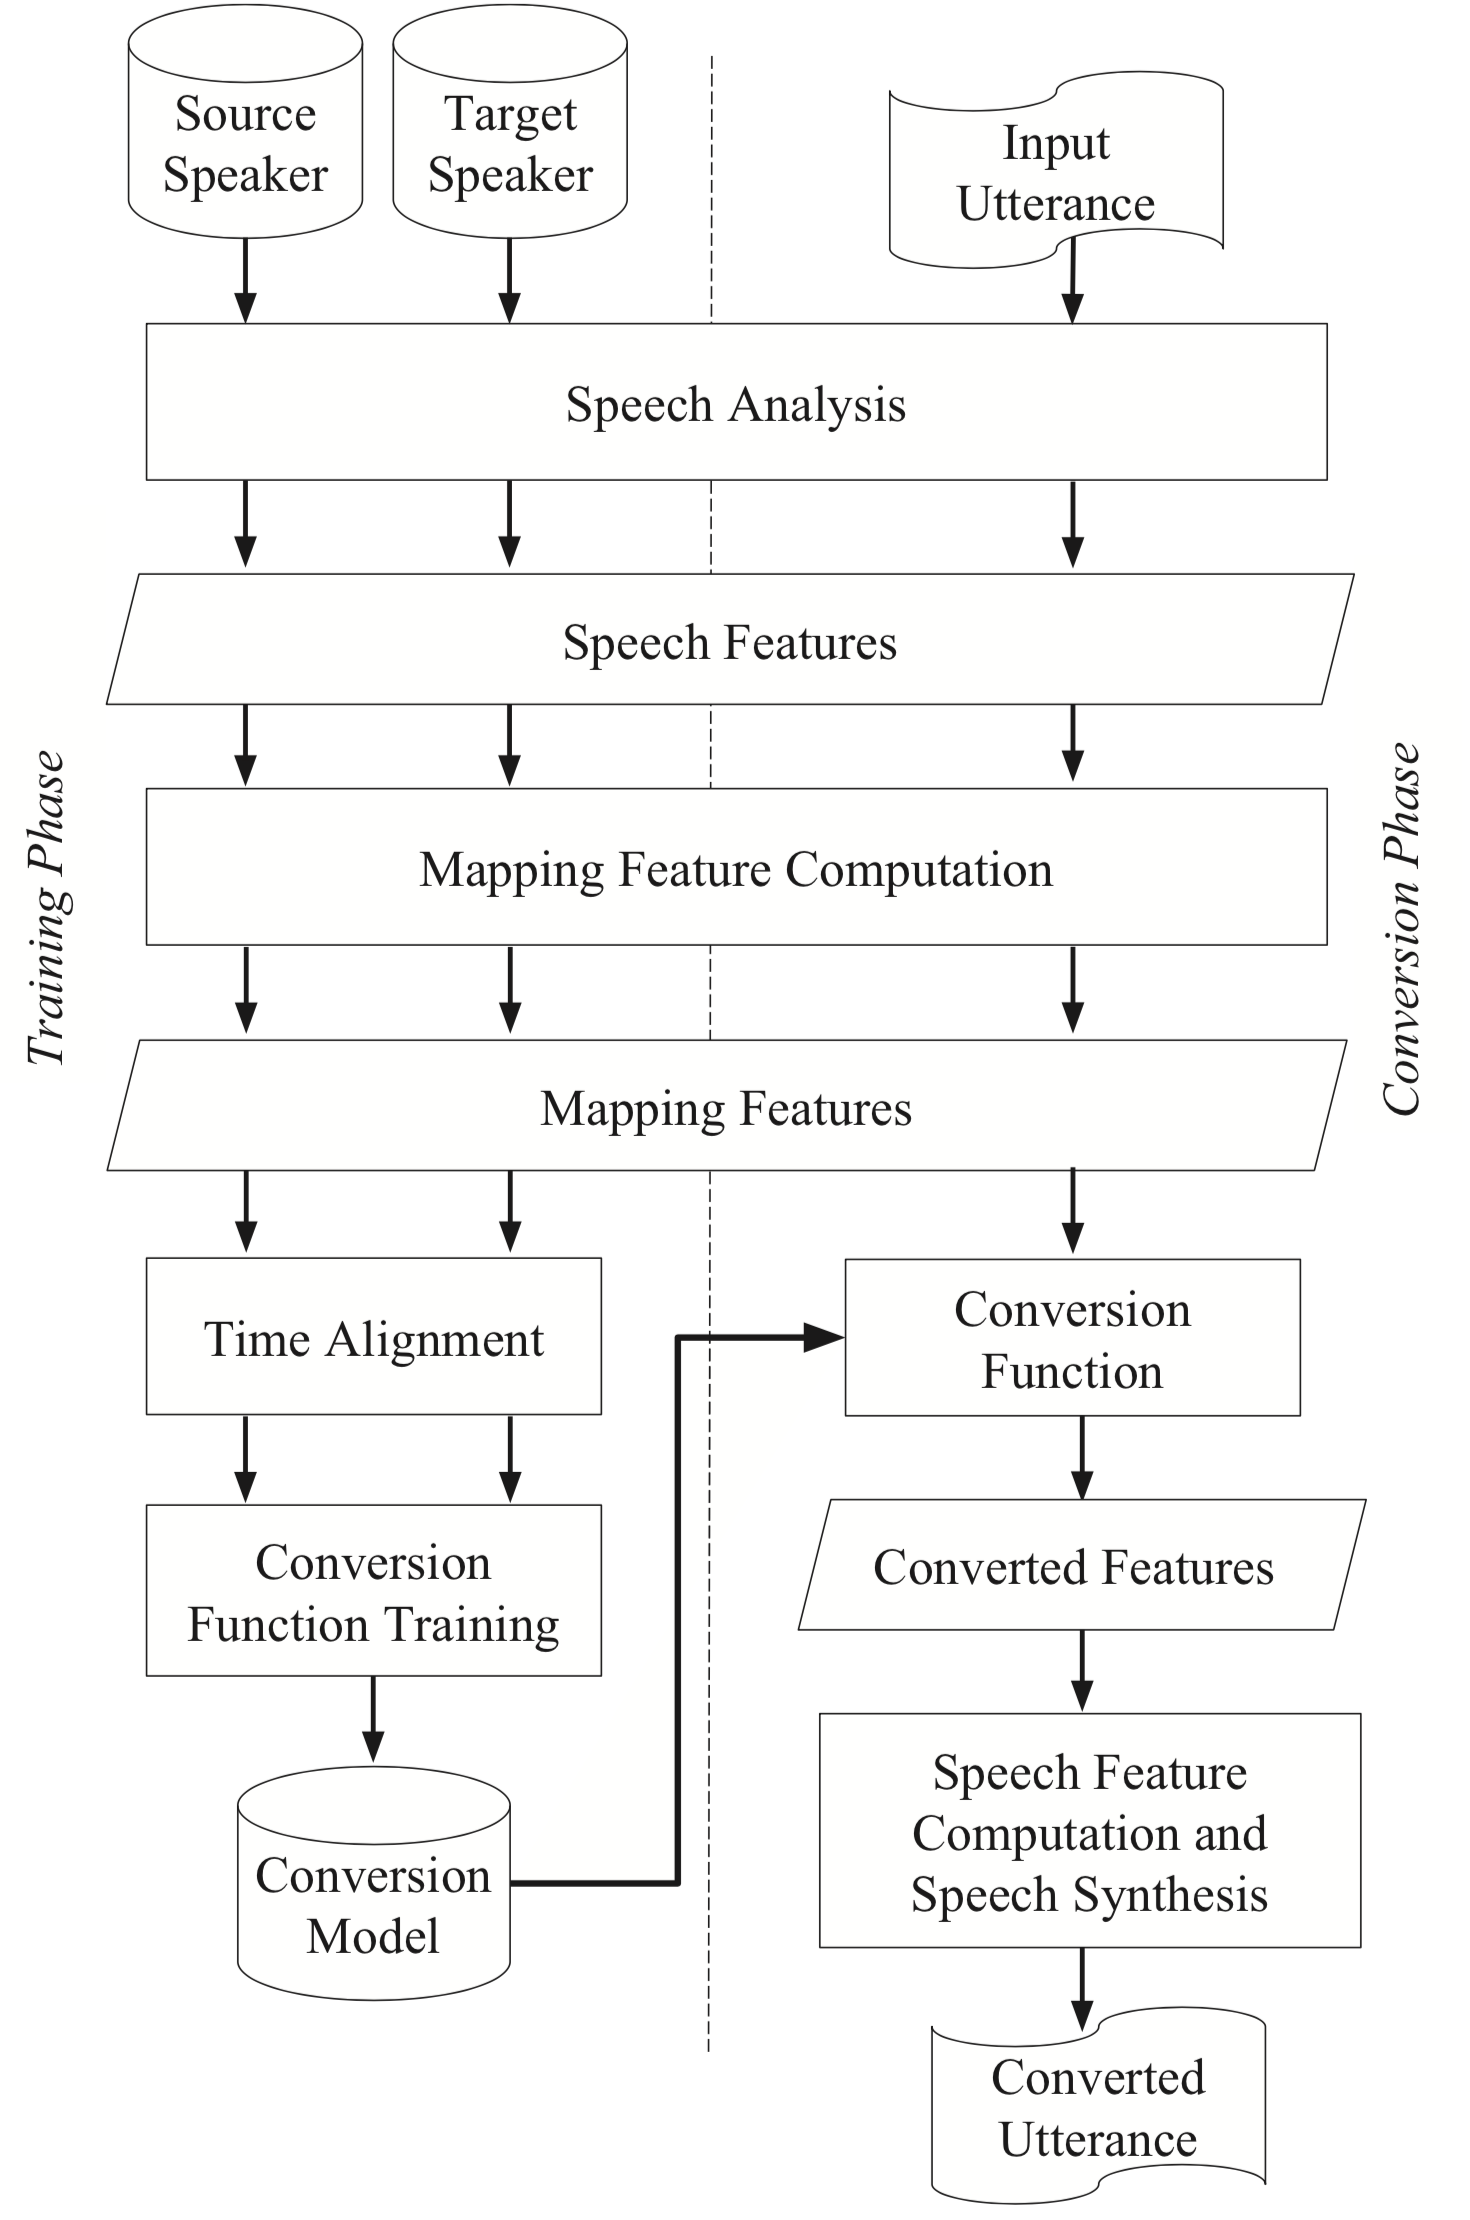
\includegraphics[scale=0.25]{img/vc-flowchart.png}
\caption{The training and conversion processes of a typical VC system. Taken from \textcite{mohammadi2017}.}
\label{fig:vc-flowchart}
\end{figure}

\hypertarget{accent-conversion}{%
\section{Accent conversion}\label{accent-conversion}}

Like voice conversion, accent conversion is dedicated to convert the
speech of a \emph{source speaker} into sounding like a \emph{target
speaker}. However, accent conversion is specifically focused on morphing
the \emph{accent} of the speech signal, as opposed to sounding directly
like the target speaker. Succinctly stated, ``Accent conversion seeks to
transform second language L2 utterances to appear as if produced with a
native (L1) accent,'' \parencite{aryal2014a}. Because the confusion that
can arise from using the terminology \emph{source speaker} and
\emph{target speaker}, the \emph{source speaker} is often referred to as
the native or L1 speaker, while the \emph{target speaker} is referred to
as the non-native or L2 speaker. This seems somewhat counter-intuitive,
but this allows for us to create a voice that retains the non-native
speaker's identity and the native speaker's accent
\parencite{zhao2018a}.

Accent conversion poses a further challenge on top of voice conversion
as the audio of the source speaker and target speaker cannot simply be
forced-aligned due to the fact that the voice quality and accent of the
target speaker would remain \parencite{aryal2014}. This means that
accent conversion may require more specialized alignment methods beyond
standard frame-by-frame alignment that can help preserve the right
speaker information while suppressing the other undesired information.
This is further discussed in the examination of previous work in accent
conversion in \autoref{accent-conversion}.

\hypertarget{technical-background}{%
\section{Technical Background}\label{technical-background}}

\subsection{Mel-frequency cepstrum coefficients}

Before any actual speech processing can happen, the speech signal needs
to be broken down into sizable and meaningful representations. This is
most traditionally done by using mel-frequency cepstrum coefficients
(MFCCs) to create vectorized representations of the acoustic
information. Although MFCCs can be extracted fairly easily using a
number of tools or available packages, there are a number of steps
required before a speech signal can be represented as a sequence of
\emph{N} number of MFCC vectors. As the feature extraction process is
heavily related to standard signal processing as well as acoustic and
articulatory phonetics, the motivation and ideas utilized to extract
features from speech signals can be extended into one large body of work
itself. In order to succinctly describe the MFCC extraction process, we
reference \textcite{jurafsky2009}.

The most common first step in feature extraction for speech signals is
referred to as \emph{pre-emphasis}. When we produce various sounds, the
energy that each sound contains is often concentrated around the lower
frequencies, which causes information in the higher frequencies to be
obstructed. This is referred to as spectral tilt and is caused by the
physiological nature of the speech production system. In order to
balance the energy in the speech signal, the speech signal is passed
through a filter which boosts the amount of energy in the higher
frequencies. In terms of signal processing, this filter is referred to
as a first-order high pass filter and can be represented using the
formula seen in \autoref{eq:pre-emphasis-filter} where \(x[n]\) refers
to the original signal and \(\alpha\) is 0.9 \(\leq\) 1.0.

\begin{equation}
\label{eq:pre-emphasis-filter}
y[n] = x[n] - \alpha x[n - 1]
\end{equation}

After the speech signal goes through pre-emphasis, the speech signal can
be separated into smaller parts such as phones or subphones. Because the
speech signal usually contains a whole word or utterance, it is
desirable to capture consistent or `stationary' points of the signal.
This is done by going over the speech signal using a process called
\emph{windowing}, where each window is assumed to contain a non-changing
part of the signal. These windows usually contain between 10ms to 30ms
of speech, and usually overlap about 30\% - 50\% with the previous
window in order to retain all of the necessary information from each
part of the signal. After the windowing process, the speech signal is
said to be split up into N number of \emph{frames}. The windowing
process can be represented using the formula seen in
\autoref{eq:windowing} where the signal \(s[n]\) is multiplied by the
window value \(w[n]\) at each time \(n\). A visual representation of the
windowing process recreated from \textcite{demarco2015} can be seen in
\autoref{fig:frame-blocking}.

\begin{equation}
\label{eq:windowing}
y[n] = w[n]s[n]
\end{equation}

\begin{figure}[]
\centering
\includegraphics[scale=0.3]{img/frame_blocking.png}
\caption{The windowing process. A reduplication of an image from \textcite{demarco2015}.}
\label{fig:frame-blocking}
\end{figure}

Even though the word `window' might suggest that its shape would be a
rectangle, a rectangular window on its own most often leads to distorted
information because of the sudden cuts that occur on the edges of the
signal. In order to address this problem, special windowing functions
such as the Hamming window, are used to decrease the values on the ends
of a frame. An example of windowing can be seen in
\autoref{fig:rect-vs-hamming}, where the hamming window can be seen
tapering off on the edges compared to the rectangular window.

\begin{figure}[]
\centering
\includegraphics[scale=0.25]{img/windowing.png}
\caption{An example of the rectangular window vs. the Hamming window on a signal. Taken from \textcite{lebourdais2015}.}
\label{fig:rect-vs-hamming}
\end{figure}

After the signal is separated into different windows, the spectral
information can be extracted using a special tool or formula known as
the Discrete Fourier Transform (DFT). This allows us to find how much
energy is in specific frequency bands. By passing the windowed discrete
signal through the Discrete Fourier Transform, we can get a complex
number that contains the magnitude and phase for each frequency
component. After the Discrete Fourier Transform, the frequencies are
converted onto the \emph{mel} scale, using a set of filters called mel
filter banks. The purpose of the mel scale is to represent human
hearing, which is more sensitive to lower pitch sounds (under 1000Hz) as
compared to higher pitch sounds. In the mel scale, sounds below 1000Hz
are placed on a linear scale, while sounds above 1000Hz are on a
logarithmic scale. The mel filter banks can be seen in
\autoref{fig:mel-filter-banks}.

\begin{figure}[]
\centering
\includegraphics[width=1\textwidth]{img/mel_filters.jpg}
\caption{Mel-filter banks. Taken from \textcite{fayek2016}.}
\label{fig:mel-filter-banks}
\end{figure}

Afterwards, the \emph{cepstrum} is calculated in order to separate
source information from filter information. From a high level, the
source-filter theory says that all sounds come from the glottis (the
area around our throat) and below, which contains information common to
all speech sounds, such as the fundamental frequency (or pitch) of
someone's voice, as well as glottal pulse information. This is compared
to the filter, which says that adjusting the vocal tract (e.g.~moving
the tongue and other articulators) define each individual sounds. By
retaining just the filter information, we can model an individual phone.
In terms of the given cepstral values, the first 12 cepstral values are
taken as they neatly represent the filter information. In terms of
signal processing, the cepstrum is calculating by using the `inverse
discrete Fourier Transform of the log magnitude of the DFT of a
signal'.The formula for calculating the cepstrum can be seen in
\autoref{eq:cepstrum}, where \(x[n]\) represents our initial signal,
\(e\) represents Euler's number (\(\sim2.718\)), \(j\) represents an
imaginary power, \(N\) represents the number of time samples from the
signal, \(n\) represents the current sample, and \(k\) represents the
current frequency between 0 and \(N-1\) Hertz \parencite{azad2017}.
While the Fourier Transform is challenging to follow mathematically,
\autoref{fig:signal-to-cepstrum} succinctly summarizes the process.

\begin{equation}
\label{eq:cepstrum}
c[n] = \sum_{n=0}^{N-1}log\bigg(\bigg|\sum_{n=0}^{N-1}x[n]e^{{-j\frac{2\pi}{N}kn}}\bigg|\bigg)e^{j\frac{2\pi}{N}kn}
\end{equation}

\begin{figure}[]
\centering
\includegraphics[width=1\textwidth]{img/signal-to-cepstrum.jpg}
\caption{The waveform to spectrum to cepstrum process.}
\label{fig:signal-to-cepstrum}
\end{figure}

Even though these steps alone could be used to model a speech signal,
additional information is often added to further better model each
frame. Among this information is energy, which can help us further
distinguish a sound, as vowels and sibilants (`breathy' sounds like /s/
or /f/) have more energy compared to stops (`hard' sounds like /k/ or
/p/). Energy is calculated using the formula seen in:
\autoref{eq:energy} where \(x\) represents the signal and \(t\)
represents a point in time.

\begin{equation}
\label{eq:energy}
Energy = \sum_{t=t_1}^{t_2}x^2[t]
\end{equation}

On top of the 12 MFCC features and 1 energy feature, features known as
deltas and double deltas are often added to represent the change in the
speech signal frame to frame. Concretely, deltas can be used to model
changes in formants or a change from stop closure to stop release.
Double deltas are then added to represent the changes between deltas,
which provide further precision in modeling an utterance. In total, this
gives us 39 MFCC features from:

\begin{itemize}
   \setlength\itemsep{-1em}
   \item{\textbf{12} cepstral coefficients}
   \item{\textbf{12} delta cepstral coefficients}
   \item{\textbf{12} double delta cepstral coefficients}
   \item{\textbf{1} energy coefficient}
   \item{\textbf{1} delta energy coefficient}
   \item{\textbf{1} double delta energy coefficient}
\end{itemize}

A visual representation of the whole MFCC extraction process can be seen
in \autoref{fig:mfcc-extraction}.

\begin{figure}[]
\centering
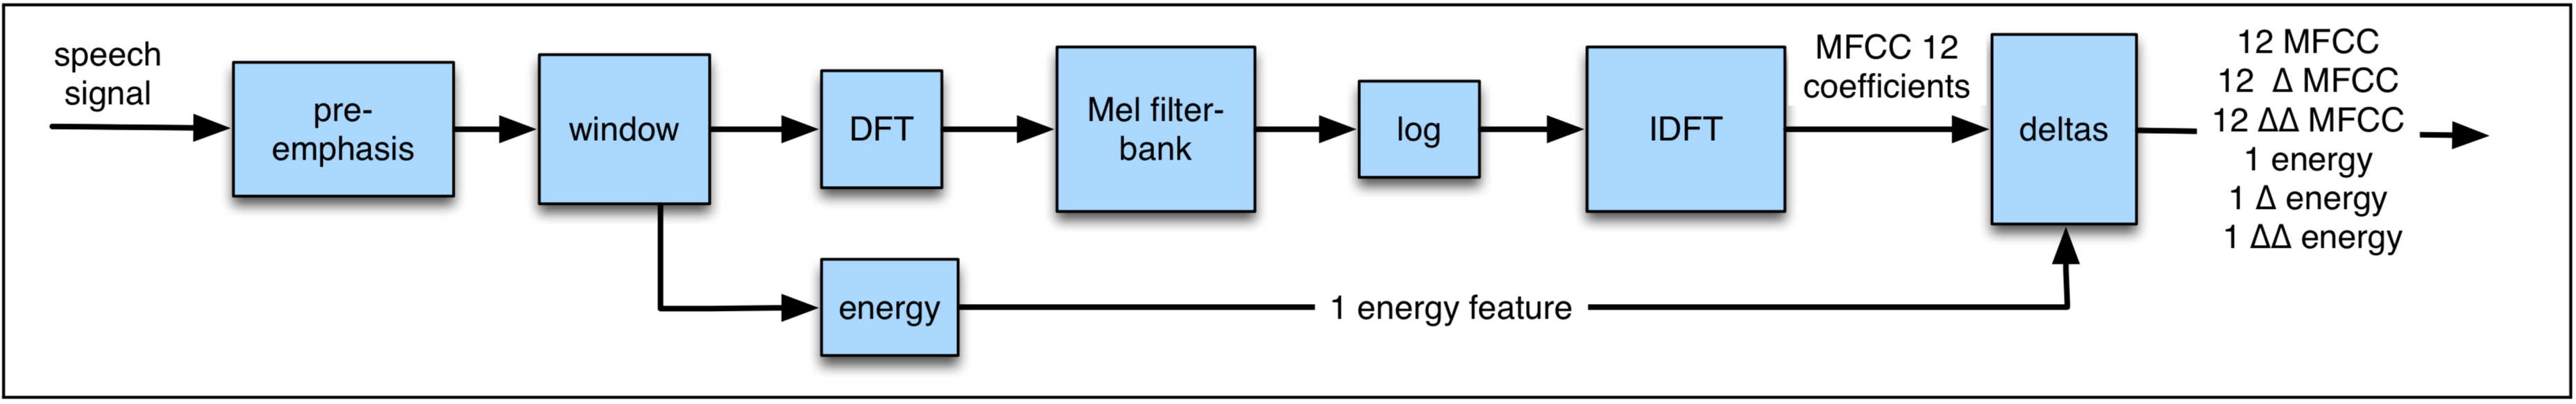
\includegraphics[scale=0.24]{img/mfcc-extraction.png}
\caption{The extraction of sequence 39-dimensional MFCC vectors from a waveform. Taken from \textcite{jurafsky2009}.}
\label{fig:mfcc-extraction}
\end{figure}

\subsection{Gaussian mixture models}

A Gaussian mixture model is a type of probablistic model that aims to
represent normally distributed groups within a set. This is based on the
idea of the normal, or \emph{Gaussian} distribution, which can be see in
\autoref{fig:gaussian-dist}. The Gaussian distribution is characterized
by two main features: the mean (the arithmetic average of the data) and
the variance (the spread of the data from the mean). The Gaussian
distribution is the most important distribution used in probablistic
modeling as it has been theorized that the average of independent random
variables would look like a normal distribution
\parencite{mcgonagle2016}.

\begin{figure}[]
\centering
\includegraphics[scale=0.40]{img/gaussian-dist2.png}
\caption{The Gaussian distribution with different means (\( \mu \)) and standard deviations (\( \sigma \)).}
\label{fig:gaussian-dist}
\end{figure}

Gaussian mixture models are based on the principle that if a unimodal
(one `peak') dataset can be fit with a Gaussian distribution, then a
multimodal (multi `peak') dataset is just a `mixture' of smaller
Gaussian distributions. A common example given to understand the
Gaussian distribution and Gaussian mixture models often references
height. It is often said that men are taller than women on average, with
men being 178cm (5 foot 10 inches), and women being 165cm (5 foot 5
inches). If we used two separate Gaussians to model each gender, we
could `mix' them to model the likelihood of a certain data point
(e.g.~person) being a male or a female \parencite{mcgonagle2016}. For
example, using a hypothetical example with the averages previously
mentioned, we could see that the likelihood of a person that is 168cm is
more likely to be a male than a female. This is demonstrated in
\autoref{fig:gmm-height}. The probabilities are calculated as the
following: the Male is P(66in) = .065 / (.065 + .104) = .38 and the
Female P(66in) = .104 / (.065 + .104) = .62, meaning that that for
someone 66 inches, it would be much more likely that they are a woman.

\begin{figure}[ht!]
\centering
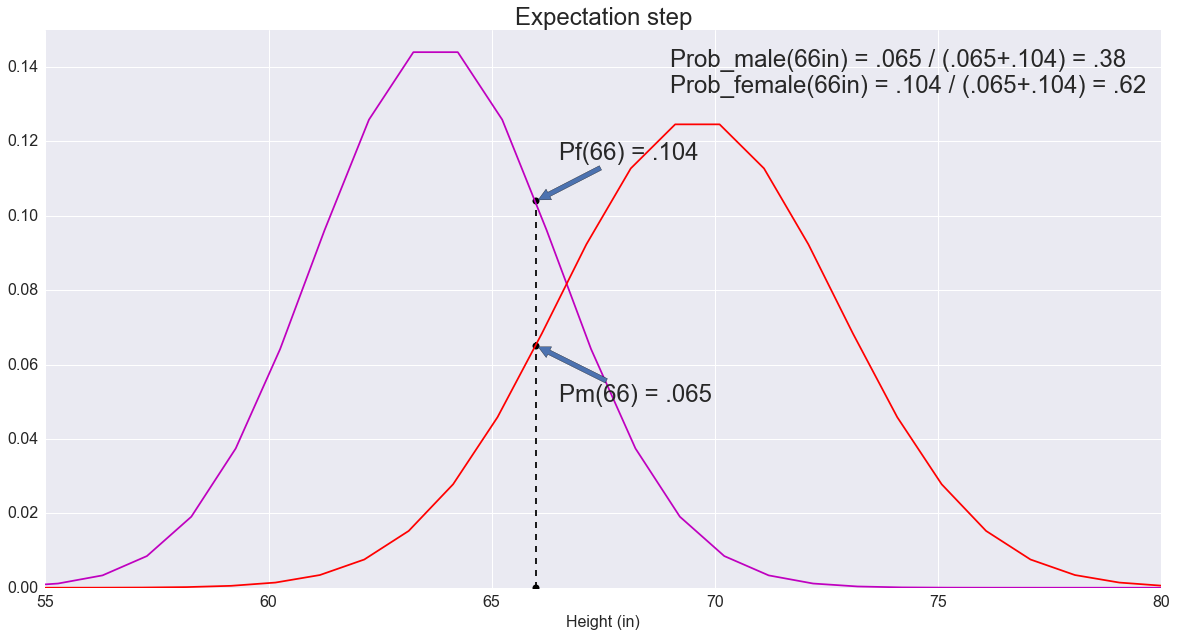
\includegraphics[scale=0.15]{img/gmm-height.png}
\caption{An example of a GMM using male and female height. The likelihoods for each gender for someone 168cm (66in) tall is calculated using the percentage of men and women in the dataset from the vertical axis.} 
\label{fig:gmm-height}
\end{figure}

However, as simple as this sounds the most advantageous point of the
Gaussian mixture model is the fact that it is an \emph{unsupervised}
model that can be used when the subpopulations of the data are unknown.
Thus, following the previous example of height, a Gaussian mixture model
could be used to model the height of the two genders \emph{without}
knowing the gender of each data point.

Because it is an \emph{unsupervised} model, it requires a special method
to estimate the appropriate parameters. The most common method used for
this is known as \emph{expectation maximization}. This algorithm is used
for maximum likelihood estimation. In mathematical terms, this can be
represented by observing the average log-likelihood to know whether the
GMM is modeling a set of vectors R well. A higher average log-likelihood
indicates that the GMM is performing well. The formula from calculating
average log-likelihood, taken from \textcite{kinnunen2009}, can be seen
in \autoref{eq:max-log-like} where \(M\) represents the number of
components, \(K\) represents the number within the codebook, \(m\)
describes the \(m\)\textsuperscript{th} Gaussian component, \(P_m\) is
the prior probability of the \(m\)\textsuperscript{th} Gaussian
component, \(\Sigma _m\) represents the co-variance matrix and
\(\mu _m\) represents the mean vector.

\begin{equation}
\label{eq:max-log-like}
LL_{avg}(R,\lambda) =\frac{1}{K}\sum_{i=1}^Klog\sum_{m=1}^{M}P_mN(r_k|\mu_m,\Sigma_m)
\end{equation}

In other words, this algorithm tries to find the most appropriate group
for each datapoint by calculating the probability of it being in a
certain group and selecting the most likely one. This is done
iteratively by initializing reasonable values, and then calculating the
probability of membership in each cluster (the \emph{expectation} step)
and updating each clusters location, normalization and shape using the
probabilities calculated (the \emph{maximization} step) until the
algorithms converge \parencite{vanderplas2016}. A visual example of the
convergence process can be seen in \autoref{fig:em-converge}.

\begin{figure}[]
   \centering
   \begin{subfigure}[b]{0.4\textwidth}
      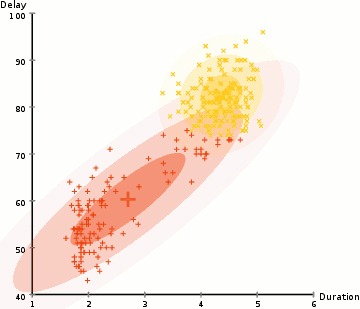
\includegraphics[width=1\textwidth]{img/em-alg2.jpg}
         \caption{Initialization}
         \label{fig:gmm-init}
   \end{subfigure}
   \quad
   \begin{subfigure}[b]{0.4\textwidth}
      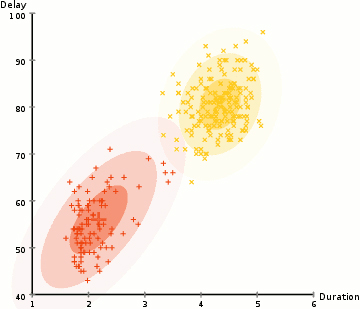
\includegraphics[width=1\textwidth]{img/em-alg3.jpg}
         \caption{Mid-convergence}
         \label{fig:gmm-mid}
   \end{subfigure}
   
   \begin{subfigure}[b]{\textwidth}
      \centering
      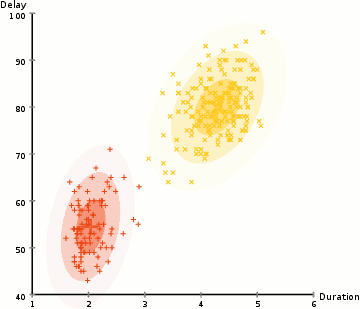
\includegraphics[width=0.45\textwidth]{img/em-alg4.jpg}
         \caption{Converged}
         \label{fig:gmm-conv}
   \end{subfigure}
   \quad
   \caption{Gaussian Mixture Model convergence using the Expectation-Maximization algorithm. Taken from \textcite{mcgonagle2016}.}
   \label{fig:em-converge}
\end{figure}

Due to the complexity of the formulas, the mathematical representations
for the expectation-maximization steps are taken from the discussion of
\textcite{demarco2015} which in turn cites \textcite{rose1990}. The
formulas are represented as follows.

\begin{enumerate}
\def\labelenumi{\arabic{enumi}.}
\tightlist
\item
  The E-Step: The posterior probabilities are calculating for all of the
  training vectors of a given class model \(\lambda\) using
  \autoref{eq:e-step}.
\end{enumerate}

\begin{equation}
\label{eq:e-step}
P(m|r_n,\lambda) = \frac{P_mN(r_n|\mu_m,\Sigma_m)}{\sum_{i=1}^MP_iN(r_n|\mu_i,\Sigma_i)}
\end{equation}

\begin{enumerate}
\def\labelenumi{\arabic{enumi}.}
\setcounter{enumi}{1}
\tightlist
\item
  The M-Step: The M-Step utilizes the posterior probabilities from the
  E-Step to estimate model parameters using
  \autoref{eq:m-step1},\autoref{eq:m-step2} and \autoref{eq:m-step3}.
\end{enumerate}

\begin{equation}
\label{eq:m-step1}
\hat{p}_m = \frac{1}{K}\sum_{k=1}^{K}P(m|r_k,\lambda)
\end{equation}

\begin{equation}
\label{eq:m-step2}
\hat{\mu}_m = \frac{\sum_{K=1}^{K}P(m|r_k,\lambda)r_k}{\sum_{K=1}^{K}P(m|r_k,\lambda)}
\end{equation}

\begin{equation}
\label{eq:m-step3}
\hat{\Sigma}_m=\frac{\sum_{k=1}^{K}P(m|r_k,\lambda)(r_k - \hat{\mu}_m)(r_k-\hat{\mu}_m)^T}{\sum_{k=1}^{K}P(m|r_k,\lambda)}
\end{equation}

\begin{enumerate}
\def\labelenumi{\arabic{enumi}.}
\setcounter{enumi}{2}
\tightlist
\item
  Set \(P_m = \hat{P}_m\), \(\mu_m = \hat{\mu}_m\), and
  \(\Sigma_m = \hat{\Sigma}_m\) and repeat the E-step and M-step until
  convergence.
\end{enumerate}

This model can be compared to the \emph{k}-means clustering algorithm,
as both can be used to cluster different subgroups. Like the
\emph{k}-means algorithm, GMMs also require us to specify a number of
components, which usually indicate the number of subgroups we hope to
cluster. However, \emph{k}-means suffers from not using a probablistic
model to assign clusters, which means that data points can only be
assigned to exactly one cluster. The cluster shape of \emph{k}-means is
also limited to only circles, which makes it inadequate to model data
with different distributions. GMMs manage to address these issues by
using the expectation-maximization algorithm to calculate the
probabilities of cluster assignment and by allowing for different
covariance types which permits for different cluster shapes beyond the
circle. Aside from being useful as an unsupervised classification
algorithm, GMMs can also be seen as a generative algorithm as it models
the overall distribution of the data \parencite{mcgonagle2016}. This
means that a GMM can be used to generate new data points following the
distribution of the given data set.

In the case of speech, Gaussian mixture models are most often used to
model individual sounds using MFCC feature vectors. The usage of
Gaussian mixture models to classify vocal features became popularized
through the work and success of \textcite{reynolds1995} . Because MFCC
feature vectors are multi-dimensional
(\begin{math} \sim \end{math}39-dimensions), the Gaussians within the
model are also multi-variate. However, the same principles described
above still stand, and allow us to calculate the probability of a sound
from a given frame. More formally, the most likely class for a an
utterance can be described using the formula seen in
\autoref{eq:gmm-calculate} taken from \textcite{oshaughnessy1999}, where
T is the test utterance and \(\lambda^n\) is the GMM.

\begin{equation}
\label{eq:gmm-calculate}
N^* = \argmax_{1\leq n \leq}P(\lambda^n|T) = \argmax_{1\leq n \leq} \frac{P(T|\lambda^P)P(\lambda^n)}{P(T)}
\end{equation}

\subsection{Neural networks}

As indicated by its name, neural networks or more formally,
\emph{artificial neural networks} are said to be based on the
architecture of the brain's neurons. Like the human decision making
process, neural networks take in a certain amount of information or
\emph{input}, to make a decision, or more formally, to give an
\emph{output}. This idea can be easily understood by taking a look at
the \emph{perceptron}, the most simple form of an artificial neuron.

\begin{figure}[]
\centering
\includegraphics[scale=0.20]{img/perceptron.png}
\caption{A visual representation of the perceptron.}
\label{fig:perceptron}
\end{figure}

A perceptron takes in a number of binary inputs (represented in the
image by \(x_1, x_2, x_3\)) and outputs a single binary output
\parencite{nielsen2015}. The output is determined by whether the inputs
are less than or greater than a defined threshold, and each input can be
weighted to represent the importance of that input in determining the
output. Mathematically, this can be represented as the following where
\(w\) represents the weight and \(x\) represents a particular value:

\begin{equation*}
    output=\begin{cases}
        0 & \text{if $\sum_{j} w_jx_j \leq$ threshold} \\
        1 & \text{if $\sum_{j} w_jx_j >$ threshold}
    \end{cases}
\end{equation*}

To provide a concrete example, we can use a yes-no question (with 0
representing `no', and 1 representing `yes') such as:

\emph{``Will I watch another episode of this TV show?''}

As `inputs', we can use the following questions:

\begin{enumerate}
\def\labelenumi{\arabic{enumi}.}
\tightlist
\item
  Do I like this show?
\item
  Is it still before my bedtime?
\item
  Am I free tomorrow?
\end{enumerate}

To decide the weights of these `inputs', we can consider how important
we think each question is. Perhaps the most important question is
Question \#1, and thus we can assign a weight of 4, while the other 2
may receive a weight of 2 and 1 respectively.

Finally, we need to define a threshold to determine whether we output a
0 (no) or a 1 (yes). Evidentally, the lower the threshold, the more
likely we're going to watch another episode. For example, with the given
weights and a threshold of 2, we have the following possible outputs for
each question:

\begin{enumerate}
\def\labelenumi{\arabic{enumi}.}
\tightlist
\item
  4 * 1 = 4 OR 4 * 0 = 0
\item
  2 * 1 = 2 OR 2 * 0 = 0
\item
  1 * 1 = 1 OR 1 * 0 = 0
\end{enumerate}

We can see that we would end up with a final output of 1 (yes) in the
case that it is still before our bedtime (2 points) and/or if we like
this show (6 points/4 points), and regardless of whether we are free
tomorrow.

Even though the previous notation of the perceptron is more simple, the
perceptron, and more generally speaking, the neuron is more often
described in the following notation where w represents a vector of the
weights, x represents a vector of the inputs, and b represents
\emph{bias}, to replace the threshold.

\begin{equation*}
    output=\begin{cases}
        0 & \text{if $w * x + b \leq$ 0} \\
        1 & \text{if $w * x + b >$ 0}
    \end{cases}
\end{equation*}

The bias can be understood as being equivalent to -threshold. It can
also be understood in terms of the neuron metaphor of how easy it is to
get the neuron to `fire'. That is to say, the bigger the bias, the more
likely we output a 1, and the smaller the bias, the more likely we
output a 0.

Although perceptrons are very simple to understand, they tend to not
function well in more complex situations due to their structure. In
particular, a small change in the weights could easily cause the output
to go from a 1 to 0 and vice versa. Of course, in the case of the
example above, this may not matter too heavily, but in training large
systems, this property is too afflicting to be reliable
\parencite{nielsen2015}.

Instead, the most basic neuron used in machine learning is the
\emph{sigmoid} neuron, which as the name indicates, utilizes the sigmoid
function to decide the threshold. This prevents the neuron from being
affected by small changes like the perceptron, as the decision function
is no longer linear. The sigmoid neuron is also much more flexible, as
it no longer requires a binary input and can instead take on any values
between 0 and 1. Aside from the sigmoid, there are other non-linear
functions that can be used, such as the tanh function or another known
as the rectified linear unit (ReLU) which can offer slight improvements
over the sigmoid depending on the task. In general, these non-linear
functions are what give neural networks their vast power to `learn'
\parencite{nielsen2015}.

While a single neuron may be able to make very basic decisions, it is
through a combination of them that we can make more complex systems that
do tasks such as named entity recognition, object detection and voice
conversion. From here, we get the name of neural \emph{network}. In
\autoref{fig:neural-network}, we see an example of a more typical neural
network.

\begin{figure}[]
\centering
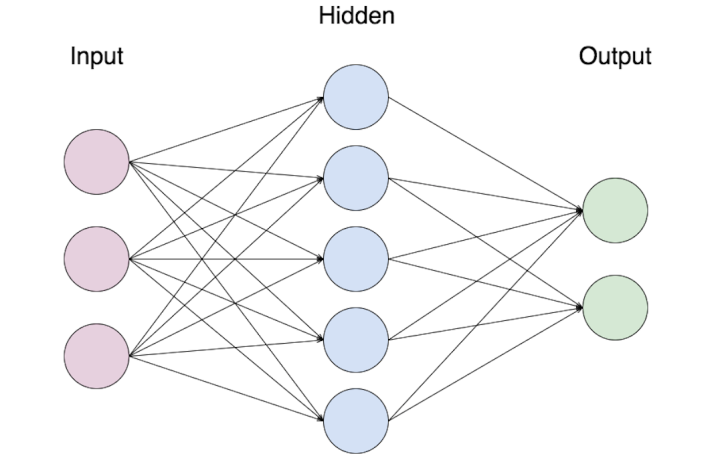
\includegraphics[scale=0.35]{img/neural-network.png}
\caption{An example of a neural network.}
\label{fig:neural-network}
\end{figure}

In the example above, we have three inputs and two outputs, and a new
concept known as a \emph{hidden layer}. The hidden layer is said to be
able to `uncover' more additional information about the input in order
to better decide the output. While the current example only has one
hidden layer, the currently popular `deep learning' comes from adding
multiple hidden layers to create a large neural network structure. Like
hidden layers, the number of inputs and the number of puts can vastly
vary depending on the dataset. For example, in the case of
part-of-speech tagging, we would like the input and output size to be
the same per sentence, as we need to have a part-of-speech tag applied
to each word. The output layer can the output the probability of each
possible part-of-speech tag (noun, verb, adjective, etc.) per word, and
we can select the most probable as that word's part-of-speech.

While neural networks are described at a high level here in order to
facilitate general understanding of this work, more complex neural
network architectures and features are not addressed here. Further
reference regarding neural networks can be found in
\textcite{nielsen2015}, the main reference for the description here, and
\textcite{goldberg2017}, which provides both an overview on neural
networks and discussion of their use in natural language processing.

Neural networks in the context of voice/accent conversion will be
further described in \autoref{accent-conversion}.
\cleardoublepage
\chapter{Literature Review}

This section provides a brief overview of second language acquisition
and education in order to frame the challenge of pronunciation and to
motivate the potential usage of technology in language learning. We
point to some previous research in spoken language technology used in
the domain of language education, including discussion on computer
assisted pronunciation (CAPT) systems in order to shed light on where
accent conversion could be applied, and then detail some important
pivotal work done in both voice and accent conversion.

\hypertarget{theoretical-and-educational-motivations}{%
\section{Theoretical and educational
motivations}\label{theoretical-and-educational-motivations}}

Linguists have long debated over the possibility of whether second
language (L2) learners (e.g.~adult learners) could ever acquire a
language to the extent of a native speaker. Some still cite ideas like
the Critical Period (CP) Hypothesis and neuroplasticity which claims
that learners cannot acquire language (at least as well as a native
speaker) after a certain point in time due to the loss of plasticity in
the brain \parencite{lenneberg1967a,scovel1988a}. This theory has been
particularly cited in reference to pronunciation, perhaps due to the
obvious difficultly in overcoming the L1 negative transfer (e.g.~effect
of our native language) that many, if not all, language learners
experience in speaking a new language.

Since the emergence of the CP hypothesis, many linguists have
investigated the relationship between a number of variables such as age,
motivation, and language use, that interact with the level of language
acquisition. \textcite{piske2001} and \textcite{lengeris2012} present an
excellent review of different literature that investigates the
interactions between these various variables and their effects on
foreign accent. They discuss that although many L2 foreign accent
studies do support the idea that the earlier a language learner learns a
language, the better their accent would be, there isn't strong enough
indication to support the notion of a `critical' period. They do concede
that many studies do indicate that there is a linear correlation between
age and foreign accent, but this only indicates a `sensitive' period,
not a `critical' period, a distinction that some fail to acknowledge.
That is to say, following advocates of the CP, the critical period
should end roughly around 12 years old \parencite{scovel1988a}, or no
later than 15 years old \parencite{patkowski1990}, and beyond this
point, there would be ``a sharp drop-off in a learner's abilities''
\parencite{lengeris2012}, indicating that a learner could not acquire a
native-like accent beyond this period.

Other researchers such as \textcite{long1990} suggested that an L2
learner could speak accent-free if they learned the language before 6
years old but not after 12 years old. Although this notion also has been
supported through a number of studies, there has also been
counter-evidence found in other studies that found that there were
learners younger than 6 who had detectable traces of a foreign accent.
In other studies that examined learners of English who started beyond 12
years old, they also found evidence of learners with no detectable
foreign accent. For example, in \textcite{flege1995}, it was found that
6\% of 120 native speakers of Italian who started learning English after
the age of 12 years old had native-like pronunciation, and in
\textcite{bongaerts1995}, it was found that 5 out of 11 speakers were
rated comparable to the native English control subjects. Thus
\textcite{piske2001} conclude that while there is evidence that earlier
learners can learn an L2 with less chance or degree of a foreign accent,
this does not necessarily support the CP hypothesis or the idea that the
loss of plasticity in the brain leads to an inability to acquire
language.

Aside from the issue of whether or not language learners could ever
achieve native-like performance, another question that arises is whether
or not there is even a \textit{need} for learners to aim so high. In
\textcite{munro1999}, they discuss the interaction between foreign
accent, comprehensibility and intelligibility and point out that the
goal for many L2 learners is to communicate and not necessarily sound
like a native speaker. Thus while there are unique groups of learners
like those from \textcite{bongaerts1995} that do achieve native-like
pronunciation, \textcite{munro1999} point out that most learners strive
for effective communication. In order to observe the interaction between
foreign accent, comprehensibility and intelligibility, a they conduct a
perceptual study on the performance of native Mandarin speakers.
Following this study, they found that despite the fact that some
speakers may have what some consider a `heavy accent', this does not
automatically mean that they are unintelligible. However, they do cite
that some accents may cause longer processing times than others. When
observing the interaction of variables such as phonemic errors and
intonation with intelligibility and comprehensibility, they found that
intonation was the most influential factor in comprehensibility, while
phonemic errors affected intelligibility. This substantiates the
concepts of comprehensibility and intelligibility themselves, as
intelligibility is the degree a speaker is understood without involving
interpretation (e.g. ``What did they say?''), while comprehensibility is
the degree a speaker is understood in terms of meaning (e.g. ``What do
they mean?''). Thus, they suggest that successful communication requires
attention to both sounds and prosody for better comprehensibility and
intelligibility.

While linguists make these discoveries and observations of L2 learning,
it seems that it takes a lot of effort for them to trickle down to the
foreign language classroom. In \textcite{darcy2012}, they find through a
small survey of 14 teachers that although teachers tend to find
pronunciation to be `very important', the majority do not teach it at
all. When asked why they do not teach it, they cited reasons such as
`time, a lack of training and the need for more guidance and
institutional support'. Even though the number of teachers surveyed may
be significantly small, this gives us a glimpse through the lens of what
language teachers themselves experience in relation to pronunciation. We
see that even though teachers would like to address it, this would
require a restructuring in their curriculum and training-- something
that would undoubtedly take even more time before students get more
pronunciation attention. Compounded with the issue of time and the fact
that not all learners need or want equal amount of pronunciation
training, it may be unlikely to see such change in second language
curriculum so soon.

This points to the potential solution of employing a technology-based
system to improve pronunciation as learners could individually address
their needs \textit{outside} of the classroom.

\hypertarget{spoken-language-technology-for-education}{%
\section{Spoken language technology for
education}\label{spoken-language-technology-for-education}}

Over the decades, as speech technology has slowly evolved and started to
show its potential, many researchers have tried to test its limits by
innovating a number of systems to address the challenge of
pronunciation. Included in these systems are systems such as
computer-assisted pronunciation training (CAPT) systems which attempt to
tutor pronunciation through explicit teaching as well as more modern
gamified techniques, which attempt to coerce language learners in to
practicing pronunciation by making the process more engaging.

Among the two, CAPT systems have had more history due to the extra
development and testing gamified techniques require. In fact, gamified
systems can be considered a subclass of CAPT systems, as both require a
fundamental setup in order to assist the language learner. In general,
these systems utilize some form of automatic speech recognition (ASR) to
record a speaker and compares their recordings (usually) with a native
speaker gold standard. They also usually include a feedback mechanism
with a combination of pitch contours, spectrograms or audio recordings
to help the user adjust their pronunciation, with gamified systems
including at least a point mechanism to motivate the user.

In order to understand the connection between language education and
spoken language technology, we take a look at \textcite{neri2002} where
we are presented with a through overview between the two areas. Here, we
see that aside from the classroom, there seems to be an issue in
relating the findings of linguistics/language pedagogy with technology.
Part of the reason, they suggest, stems from the fact that there are not
`clear guidelines' on how to adapt second language acquisition research
and thus many CAPT systems `fail to meet sound pedagogical
requirements'. They emphasize the need for the learners to have
appropriate input, output, and feedback and exhibit how the systems
available at the time were lacking. For example, they criticize some
CAPT systems that were prevalent at the time including systems like
\textit{Pro-nunciation} and the \textit{Tell Me More} series for
utilizing feedback systems that give the users feedback in waveforms and
spectrograms, which cannot be easily interpreted without training.
Further, they argue that although visual feedback has its merits, this
kind of feedback suggests to the user that their utterance must look
close to what is shown on the screen, which is not the case. An
utterance can be pronounced perfectly fine, but look completely
different from a spectrogram, and \textit{especially} a waveform due to
the number of features represented in each visualization, such as the
intensity, which will indefinitely vary from user to user and the given
examplar. They conclude their article by making it a point to discuss
recommendations for CAPT systems, by stating that they should integrate
what has been found in research from second language acquisition, and to
train pronunciation in a communicative manner to give context to the
learners. They also point to the problematic area of feedback and advise
that systems provide more easily interpretable feedback with both audio
and visual information, and propose that systems give exercises that are
`realistic, varied, and engaging'.

While \textcite{neri2002} makes solid recommendations in improving CAPT
systems, building pronunciation systems that take all of the previous
suggestions into consideration requires adept planning and expertise,
and can be demanding for most research groups. Instead, some of have
tried to adapt already existing technology and build a small
architecture around it. For example, \parencite{tejedor-garcia2017}
experiment with utilizing synthetic voices for corrective feedback in a
pronunciation training tool. In their study, they use Google's offline
Android text-to-speech (TTS) system as feedback for B1 and B2 Spanish
learners of English, and have them focus on the six most difficult pairs
of vowels. In order to train the users, the researchers first had them
watch videos that describe the articulatory/perceptive features of the
vowels, and had them listen to a number of minimal pairs produced by the
TTS system in succession. Afterwards, they were asked to discriminate
minimal pairs in a listening task and then asked to pronounce them. From
this study, they conclude that making use of commercial TTS systems are
beneficial for users and instructors alike as indicated by both the
improvement in performance by the users and the feedback given by those
involved in the experiment. However, because the study was limited to
individual words and only six pairs of vowels, further experimentation
needs to be conducted in order to understand whether these learners can
generalize their training.

While a brief overview, it is evident that there is a large potential
for appropriately adapting technology to guide and help language
learners and teachers alike. Yet, in order to provide long-standing
worthwhile results, further consideration needs to be given to the
suggestions and evidence of previous research and should be integrated
in the design and implementation of future systems. This implies that
the appropriate time and resources may need to be dedicated in order to
push the boundaries of technology and its application in language
education.

\hypertarget{voice-conversion}{%
\section{Voice conversion}\label{voice-conversion}}

There have been a number of efforts to design voice conversion systems
using various methodologies. Much like the rest of the speech technology
field, earlier voice conversion systems began with utilizing MFCCs and
GMMs for conversion and slowly evolved towards utilizing more advanced
features and adaptation techniques.

In particular, a variation of GMM voice conversion set forth by
\textcite{toda2007} has become what appears to be the standard set-up.
Following their reasoning, they argue that although regular GMMs perform
fairly well in voice conversion, they also lead to the deterioration of
speech quality. Instead, they propose that by using a maximum-likelihood
estimation of the spectral parameter trajectories, issues that cause the
loss of quality such as oversmoothing of the spectral features can be
avoided. They provide detailed theoretical evidence to support their
method which can be further observed by taking a look at their paper.

GMMs have long been used for voice conversion alongside other speech
tasks, but more recently another method-- or more accurately another
feature in place of MFCCs, known as \emph{i-vectors} have taken off. To
put concisely, i-vectors are akin to word embeddings in text-based
natural language processing tasks in the sense that i-vectors
encapsulate any type of desired speech information in a vectorized
fashion. This may be confusable with MFCCs, which also vectorize speech
information; however MFCCs specifically vectorize individual speech
sounds from frames, while i-vectors tend to vectorize more large-scale,
dynamic speech information.

The usage of i-vectors have proven to be successful in a number of
tasks, such as speaker verification, language identification, and native
accent identification. They have become especially popular due to the
fact that they work well with unlabeled acoustic data. Referring back to
the overview of voice conversion in the previous section, it is
mentioned that labeled acoustic data often leads to better results in
the conversion, but is also often unavailable. Thus i-vectors are able
to fill this gap in the lack of available labeled data and the loss of
conversion quality.

In the instance of voice conversion, i-vectors are made of speaker
super-vectors trained on GMMs and low dimensional features that
represent an individual speaker's features \parencite{wu2016}. This is
extracted per utterance and then averaged to form an i-vector that
represents an individual speaker. In this way, a source speaker's
i-vector can be approximated towards a target speaker's i-vector by a
mapping function using neural networks, gaussian mixture models, or
other appropriate algorithms.

The usage of i-vectors in voice conversion has been seen in works such
as \textcite{wu2016} and \textcite{kinnunen2017}. Following
\textcite{kinnunen2017}, the usage of i-vectors in voice conversion
aligns perfectly with the task as it is highly similar to speaker
verification; however instead of being a classification task (e.g.~is
this said speaker or not), voice conversion is a regression task. In
\textcite{wu2016}, they test and compare the performance of using plain
mel-cepstral coefficients (MCCs) against i-vectors by training a variety
of systems. Among their systems, they utilize a strategy known as the
\emph{average voice model}, which models what an average speaker would
sound like by utilizing a large amount of parallel utterances, which
also allows for conversion between two speakers \emph{without} having
parallel utterances. In order to compare MCCs vs.~i-vectors, they train
systems using MCCs as features with a deep bi-directional long-short
term memory neural (DBLSTM) network architecture, a DBLSTM combined with
an average voice model (DBLSTM + AVM), and a DBLSTM combined with an
average voice model retrained on some paralleled data from the testing
source-target speakers (DBLSTM + RM). They then train another system
with i-vectors using the DBLSTM and average voice model (DBLSTM + AVM +
i-vectors). In order to evaluate these models, they provide both an
objective evaluation using a measure known as mel-cepstral distortion
(MCD) and a subjective evaluation rated on quality and similarity, which
was decided by the votes of 20 listeners.

Following the results of the objective evaluation, they find that the
system with the lowest mel-cepstral distortion (e.g.~the best system) is
the DBLSTM + RM model, followed by the DBLSTM + AVM model, with the
regular DBLSTM system and DBLSTM + AVM + i-vector system performing
roughly the same. They note that the DBLSTM + RM system likely performed
the best because of the inclusion of parallel data from the test
dataset, while the DBLSTM + AVM outperformed the regular DBLSTM likely
due to the size of the training data. However, they do not give much
indication as to why the DBLSTM + AVM and DBLSTM + AVM + i-vectors
perform similarly. Based off of the MCD alone, it would seem that
i-vectors do not provide much benefit; however they emphasize that the
DBLSTM + RM system does include parallel data while the DBLSTM + AVM +
i-vectors system does not.

In the subjective evaluation, they compare the four systems by using an
ABX preference test to compare: DBLSTM + RM vs.~DBLSTM, DBLSTM + AVM +
i-vectors vs.~DBLSTM + RM and DBLSTM + AVM + i-vectors vs.~DBLSTM + AVM.
With each pair, they have the listeners evaluate 10 sentences for a
total of 200 votes for each system. Following the results, they find
that the DBLSTM + AVM + i-vectors system outperforms the DBLSTM + AVM
system in both the speech quality and speaker similarity categories with
statistical significance, which shows that the average voice model
\emph{without} i-vectors (e.g.~MCCs only cannot capture speaker specific
information. They also find that the DBLSTM + RM system outperforms the
plain DBLSTM system with statistical significance, indicating that the
average voice model is not only useful, but also helps reduce the amount
of parallel training data required to improve the performance. Finally,
they find that the DBLSTM + AVM + i-vectors system was rated slightly
higher in quality, but opposite in similarity. However this was without
statistical significance, indicating that they perform roughly the same.
From this study, \textcite{wu2016} concludes that the DBLSTM + AVM +
i-vectors method has potential as it allows for great flexibility to
generate the target speaker spectrum without using parallel data.

\textcite{demarco2013}, present a through analysis of the usage of
i-vectors in classifying native British accents using the same ABI
corpus utilized in one of the experiments of this work. When comparing
more traditional classifiers such as a universal background GMM, a
support vector machine with GMMs, GMMs with unigrams/bi-grams to various
i-vector configurations, \textcite{demarco2013} found that utilizing
i-vectors outperformed the traditional methods by as much as 25\%.

Even though systematic objective and subjective evaluation against older
methods do indicate that recent methods have improved upon the older
ones, comparing the performance of these systems against a true human
voice, or perhaps more fairly, against other recent systems in other
areas of speech technology, these systems still seem to leave a lot left
to be desired. For example, in listening to the audio of
\textcite{wu2016}\footnote{Visit http://www.nwpu-aslp.org/vc/apsipa-jiewu-demo.pptx to hear samples.}
it is apparent that regardless of the low quality of the original source
and target audios, the quality of the converted audio sounds muffled.
This can be attributed to the various nuanced steps and features
required to have high quality voice conversion.

For example, in a shared task dedicated to voice conversion,
appropriately called \emph{The Voice Conversion Challenge} where many
leading research groups involved in speech technology around the world
have submitted systems in attempts to tackle the issue. In the second
iteration of the challenge \textcite{lorenzo-trueba2018}, the organizers
proposed both a parallel and non-parallel version of the task, both of
which were evaluated on natural and similarity using crowdsourcing.

The type of systems submitted to the 2018 edition of the task displays
the current state of voice conversion and perhaps machine learning
research in general as this year saw a huge increase in the number of
systems using neural networks. However, it does not go without saying
that there were indeed systems that used more traditional statistical
methods, such as Gaussian Mixture Models (GMM) and one of its
variations, differential GMM (DIFFGMM).

In order to evaluate the systems, a group of roughly 300 listeners were
gathered to carry out a perceptual evaluation. The systems were
evaluated on two main measures: naturalness, which was evaluated on a
scale of 1 (completely unnatural) to 5 (completely natural); and
similarity, which was evaluated using a same/different paradigm.
Following the results, only one system, referred to as N10, was able to
outperform the baseline in terms of naturalness (alongside the original
source and target audios). When observing the performance of other
systems in terms of similarity, we see about 5 our of 23 submitted
systems outperforming the baseline. From this, we can conclude that it
easier to create a system with high similarity than high naturalness,
which is consistent with other common systems.

In discussing the results of the N10 system, the authors credit the
success of the system to the \emph{hundreds of hours} of external speech
data that was utilized to train a model to recognize content-related
features, as well manual fine-tuning. The creators of this system also
made use of WaveNet, a novel high-fidelity vocoder and dozens of hours
of clean English speech, which could also explain the success of their
results. Thus, as previously discussed, we can conclude that creating a
high-fidelity voice conversion requires not only appropriate fine-tuning
of the data, but also a large amount of external data to support the
system.

Thus, even though many systems were neural network based, only one
neural network based system was able to outperform the sprocket
GMM-based baseline, which could suggest that NN-based methods require
proper fine-tuning of the hyperparameters.

Although we see limitations in the systems presented in The 2018 Voice
Conversion Challenge, there have been other efforts to present high
quality voice conversion systems in works such as and
\textcite{nguyen2016} and \textcite{fang2018}. For example, in
\textcite{fang2018}, they leverage a cycle-consistent adversarial
network (CycleGAN) architecture, a variation of the recently trending
generative adversarial network (GAN) architecture, which was originally
used for unpaired image-to-image translation.

While not necessarily directly related to the standard idea of voice
conversion, there have also been some incredible breakthroughs in
systems set forth by research teams at Google Brain. One such system
involves the Tacotron end-to-end system, which has been proposed to
replace the current set-up of text-to-speech systems by reducing the
amount of components (decoder, vocoder, etc.) into one piece. The
researchers working on this system have recently revealed a impressive
system that also takes advantage of deep neural networks to encode
speaker characteristics into embeddings, which are then utilized to
transfer style \parencite{wang2018}. They show how their system is
capable of transferring a variety of emotions and accents, making the
synthesized audio sound more human-like. Samples of these audios can be
found at the following
link\footnote{Visit \url{https://google.github.io/tacotron/publications/global_style_tokens/} to hear samples.}.

Even though the these systems created by Google Brain are highly
impressive, it is evident that the reason for the success of their
systems is due to very fine-grained parameter tuning and the
availability of large-scale, high quality data that many research
institutions likely do not have access to or have funding for. For
example, if we juxtaposed the audio from the Google Brain systems to the
best performing system of the Voice Conversion Challenge 2018, we can
still observe some disfluencies in the audios of the best system of the
VCC 2018. Thus, it may be a long while before the general public has the
ability to completely replicate such systems and before this work
trickles in to the domain of accent conversion.

\hypertarget{accent-conversion}{%
\section{Accent conversion}\label{accent-conversion}}

Due to the specialized nature of accent conversion as compared to voice
conversion, there are fewer articles and systems available for
reference. In fact, most of the recent articles that are easily
accessible on accent conversion were all published by the same group of
researchers at Texas A\&M University.

However, before the work of these researchers, works such as
\textcite{yan2004} and \textcite{huckvale2007}, explored manipulating
various features in order to observe their relationship with a perceived
accent. In \textcite{yan2004}, they manipulate spectral features,
intonation patterns and duration in order to observe their correlation
across British, Australian and American accents. Through an ABX
perceptual test, they found that 75\% of the synthesized utterances were
evaluated as having the native accent, highlighting the potential for
segmental accent conversion.

In \textcite{huckvale2007}, they examine the relationship between
intelligibility and the of morphing various segmental and suprasegmental
features such as pitch, rhythm and segments of an English TTS system
designed to speak `accented' Japanese. This TTS system was designed by
creating a custom dictionary and mapping the Japanese sounds to their
closest English counterpart. They found through native speaker
evaluation that morphing pitch and rhythm individually had no effect,
and similarly modifying segments alone only gave a small improvement.
However, they discovered that combining the morphing of all of these
features created a large increase in intelligibility, with
intelligibility going up from 57\% as seen in their lowest-performing
system to 84\%. The results emphasize the need to consider the
interaction between segmental and suprasegmental in the conversion task.

In one of the earliest works from the Texas A\&M research group, and
perhaps a key influential paper to this work, \textcite{felps2009}
examines the potential of using a method known as Pitch-Synchronous
Overlap and Add (PSOLA) for accent with the motivation of applying it in
the context of language learning. Specifically, they utilize a
specialized PSOLA method known as Fourier-domain PSOLA (FD-PSOLA), as it
performs best in preventing spectral distortion when modifying the
pitch. In order to conduct the conversion process, they separate the
converting of the segments and the converting of the prosody into two
separate parts, with both parts evaluated individually and combined. In
evaluating their method, they measured the accentedness, acoustic
quality and identity of each converted audio using auditory tests given
to a number of speakers. Similar to \textcite{huckvale2007}, they
observe that the combination of prosodic and segemental transformation
lead to a large improvement in reducing foreign accent. However, in
terms of quality, they found that all transformations led to lower
ratings, which likely indicates the loss of some spectral information.
The identity ratings proved to be the most interesting as
\textcite{felps2009} find that the listeners indicate a `third' speaker.
In other words, the converted audio sounds neither like the source or
target speaker. Thus \textcite{felps2009} concludes that while
accentedness is reduced by their system, their proposed system also
loses the necessary information needed to retain the speaker's identity.

In other works done by this group of researchers such as
\textcite{aryal2014}, they continue to make efforts to address this
challenge. Throughout their research, they test a variety of
methodologies, including accent conversion through voice morphing and
articulatory synthesis. In \textcite{aryal2014}, they propose a
variation to standard forced alignment techniques used in voice
conversion to pair frames based on acoustic similarity.This particular
paper serves as the main basis for the experiments and research
conducted in this work due to its relative ease compared to some of
their earlier and later work.

Following their methodology, they first use dynamic time warping (DTW)
to align parallel utterances from the L1 and L2 speakers in order to
apply vocal tract length normalization to dampen the differences in
pitch. They then extract sequences of 24 MFCCs per utterance, and
cluster the MFCC vectors into 512 clusters using the \textit{k}-means
algorithm to easily find the most acoustically similar sound for each
frame. The most acoustically similar frames are then calculated by
finding the closest L2 cluster, and then selecting the most similar
frame within the cluster. After the closest vectors are paired, they map
the conversion using a GMM.

In order to evaluate their system, they had a group of 13 participants
rate 12 utterances from the test set for their perceived accent (Which
utterance was less accented?) and perceived speaker identity (Does
utterance X sound more similar to A or B?). This system was compared to
a standard voice conversion system that uses standard forced alignment
and trained using GMMs. They found that comparing the AC system to the
original L2 audio resulted in participants rating the converted audio as
sounding less accented 86\% of the time, while the VC system compared to
the original L2 audio was rated at 91\% of the time. However, when the
converted audios from both systems were compared, participants rated the
AC system to be less accented compared to the VC system 59\% of the
time. It was also concluded that the AC system was more successful in
retaining speaker identity, as the participants found the converted
audio more similar to the L2 speaker 78\% of the time. More
interestingly, they found that the AC system was especially effective in
converted utterances that are harder for the L2 speaker to pronounce.
This was measured by examining the relationship between the number of
phonemes that do not exist in the L2 language (in this case Spanish),
and the number of listeners who judged the converted speech as sounding
less accented.They found that there was a 0.86 correlation, indicating
the robustness of the AC system. Thus, it appears that adjusting the
alignment method to align acoustically similar sounds is a good start
for accent conversion systems.

In \textcite{aryal2014a} and \textcite{aryal2015}, we see a more novel
method that looks beyond acoustic features to perform accent conversion.
Citing the results of their previous work, they motivate the usage of
articulatory gesture information in accent conversion reasoning that
acoustic-based systems often struggle in the challenge of separating
accent from speaker identity, which causes the accent converted audio to
sound like a combination of the L1 speaker and L2 speaker. In order to
test this idea, in \textcite{aryal2015}, they propose a system that
combines both the more standard acoustic information like aperiodicity,
pitch and energy from the L1 speaker with articulatory information
recording using an electromagnetic articulograph (EMA). Like many recent
works, they test a DNN-based mapping function between the L1 and L2
data, which they compare to the previously popular GMM-based system.

In the evaluation of their system, they again use crowdsourced efforts
to rate their system based on intelligibility, accentedness, and speaker
identity. According to their sample size of 15 participants, they find
that the DNN-based system was rated to have a 4.3 out of 7 in terms of
intelligibility as compared to 3.84 out of 7 for the GMM-based system,
proving that including articulatory gesture information and DNNs are
more robust in this instance. The participants also rated the DNN-based
system to be more native-like in 67\% of cases as compared to the
GMM-based system. With that said, the test set was only 15 sentences,
which indicates that 10 out of 15 sentences were better with the DNN
system; thus the test set used may be too small to draw hard
conclusions. The most important conclusions drawn from their experiments
was that of the voice identity assessment. In asking the participants to
rate whether an MFCC compression and AC audio from the DNN and GMM-based
systems, they found that the participants were fairly confident that the
two audios were from the same person with both systems, with the
DNN-based system outperforming the GMM-based system as before at a score
of 4.3 out of 7 on average, and the GMM-based system at a score of 4.0.
However, this is difficult to compare to more common acoustic-only
accent conversion systems, as this is not including in their evaluation.
With that said, it may be possible to conclude that this would
outperform acoustic-based systems, as they proposed this system to
tackle flaws in their previous work.

Evidentally, although including articulatory gesture information seems
to improve the performance of accent conversion systems, as discussed in
the closing remarks of their paper, recording articulatory gesture
information can cost a great deal of money and time
\parencite{aryal2015}. Most publically (and privatized) speech corpora
also do not include this type of information, meaning that experimenting
with it in accent conversion at a broader scale is unfeasibile. Thus, it
is ambitious to accept adding articulatory information to accent
conversion systems and further work needs to be done in order to scale
standard audio-based speech corpora.

Departing from utilizing articulatory gesture information,
\textcite{zhao2018a} returns to a more simpler method similar to
\textcite{aryal2014}. However, instead of matching frames based on their
\emph{acoustic} similarity, they test matching frames based on their
\emph{phonetic} similarity. They do this by mapping the frames of each
source and target speaker into something referred to as a \emph{phonetic
posteriorgram}. Following \textcite{hazen2009}, a phonetic posteriorgram
is `a time vs.~class matrix that represents the posterior probability of
each phonetic class for each time frame'. An example of a phonetic
posteriorgram taken from \textcite{hazen2009} can be seen in
\autoref{fig:phonetic-postgram}.

\begin{figure}[]
\centering
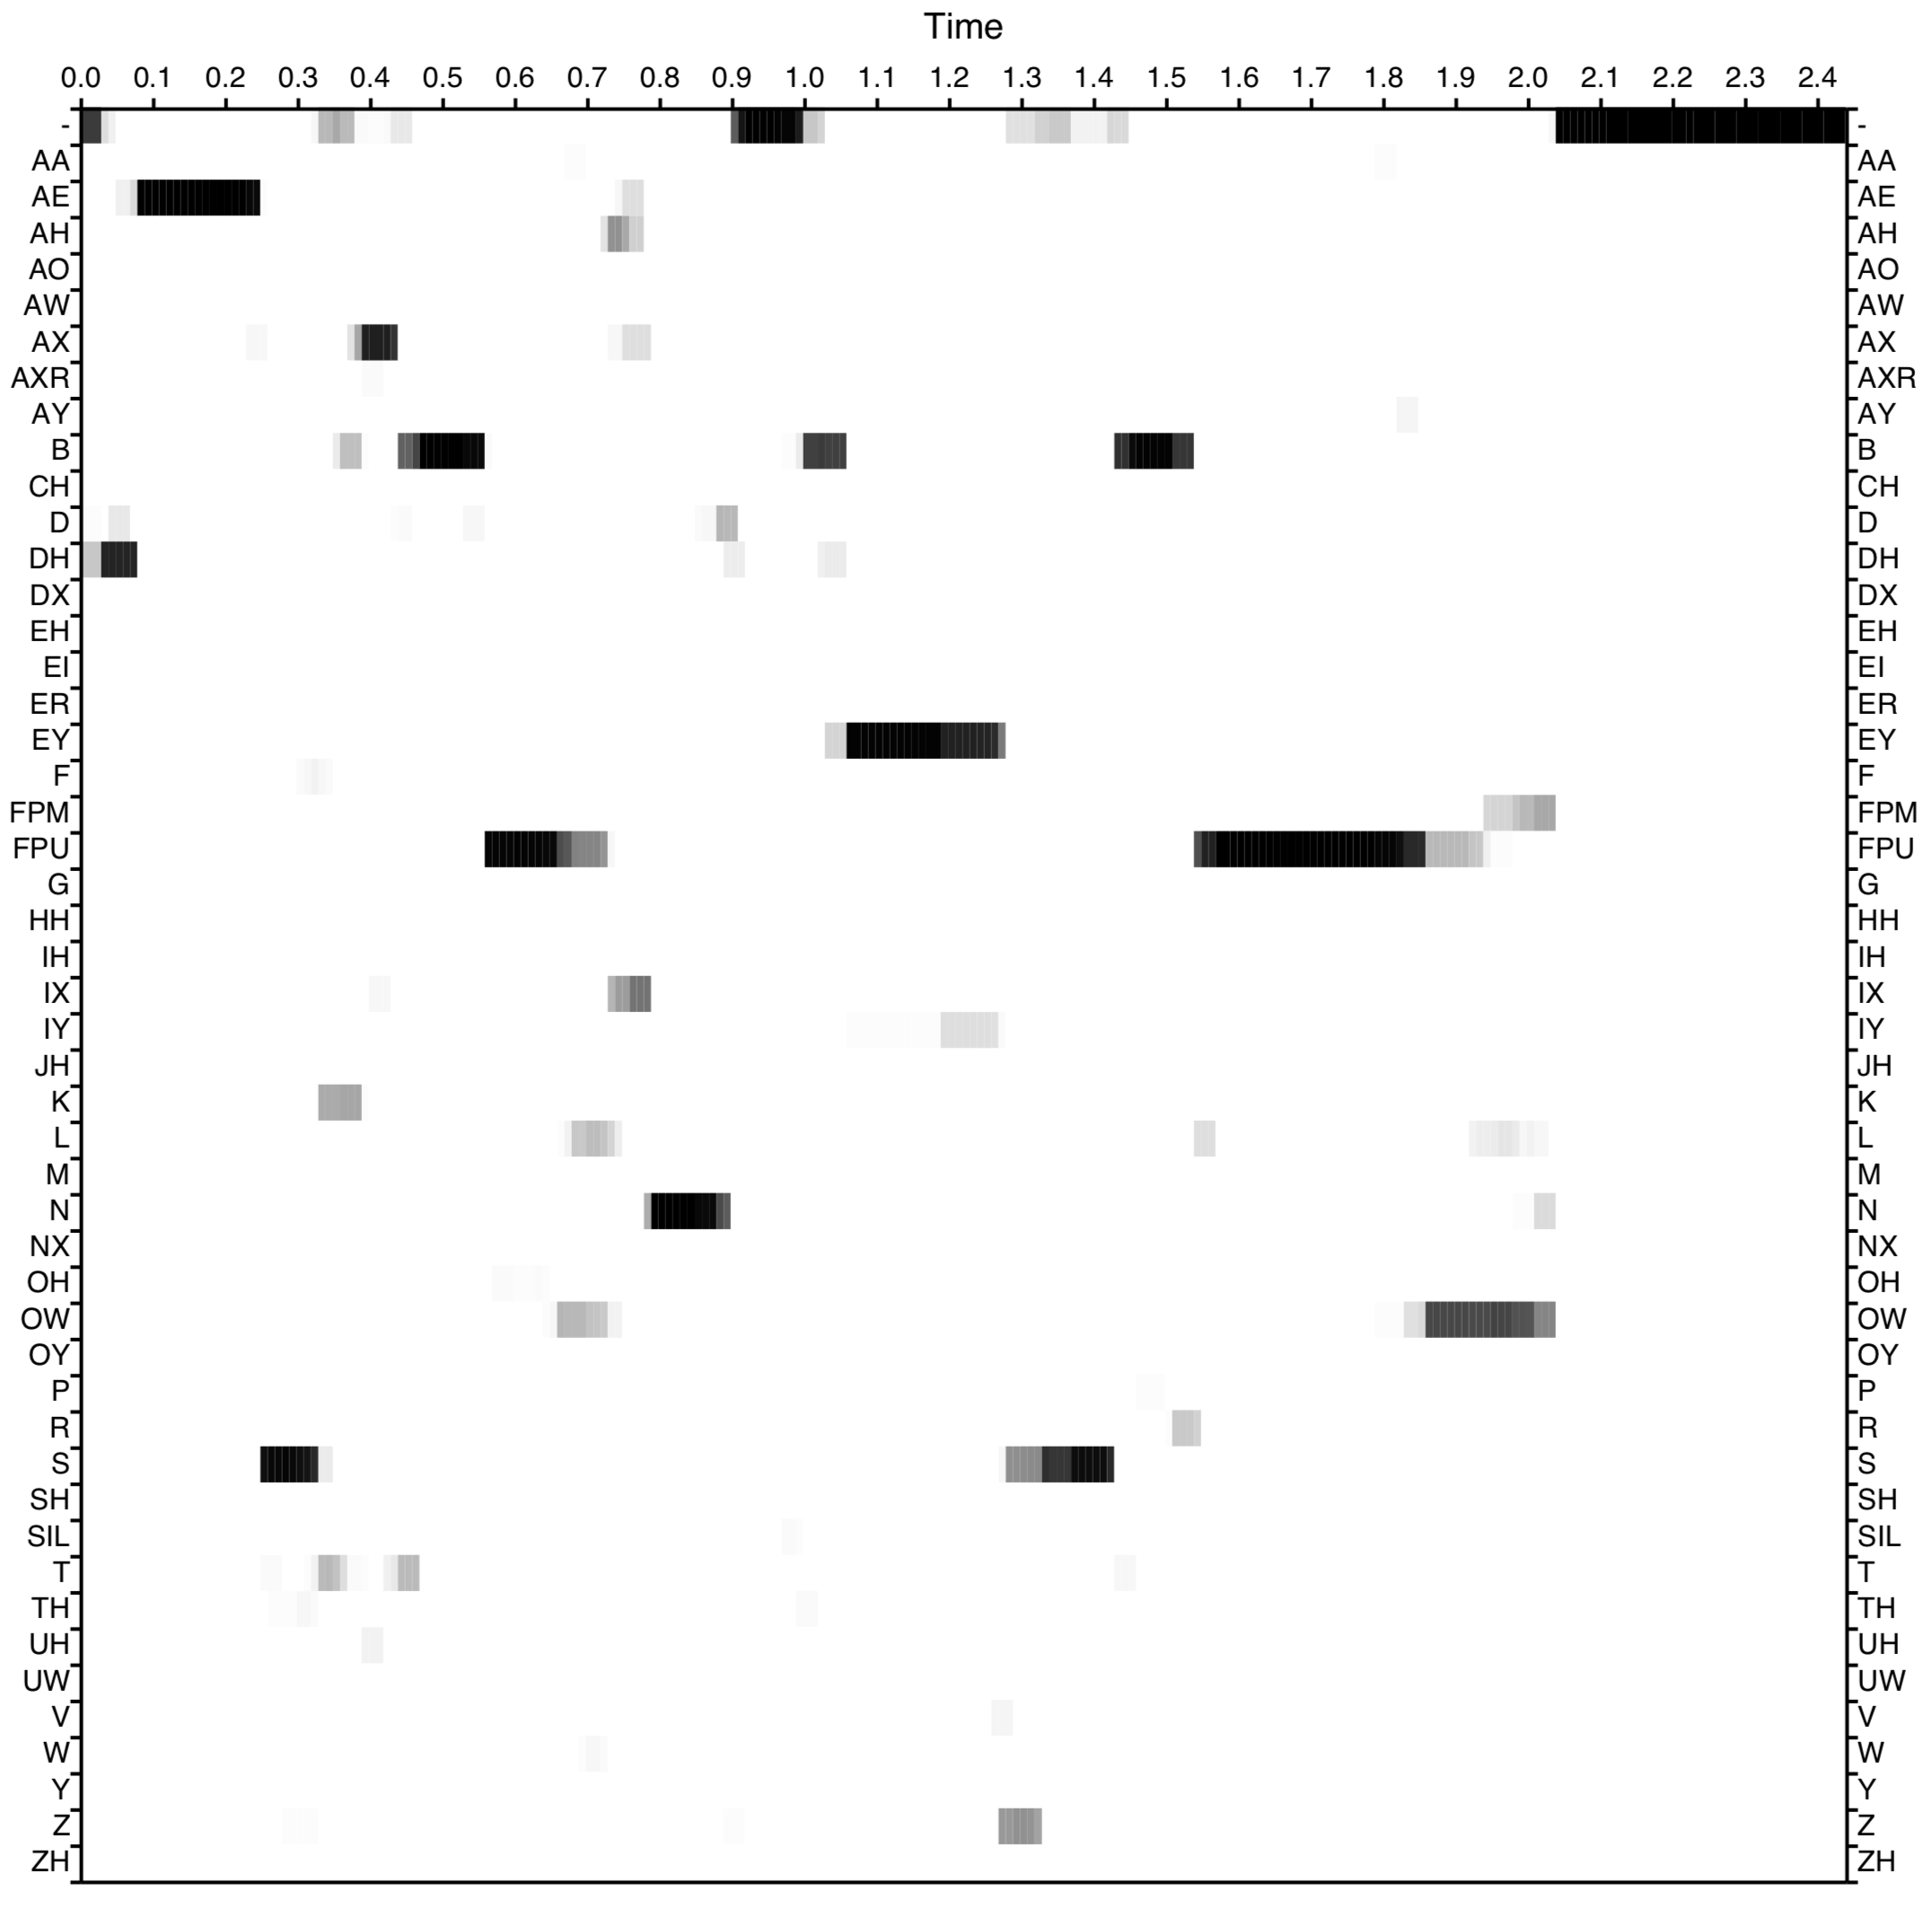
\includegraphics[scale=0.22]{img/phonetic-postgram.png}
\caption{An example posteriorgram representation for the spoken phrase `basketball and baseball'. The x-axis represents the time across the utterance and the y-axis represents the possible phonemes. Taken from \textcite{hazen2009}.}
\label{fig:phonetic-postgram}
\end{figure}

The phonetic posteriorgrams are computed using a native English
speaker-independent acoustic model and then the most similar source and
target frames are matched by calculating something known as the
Kullback-Leibler divergence (0 indicating similar or same behavior, 1
indicating completely different) between the source and target
posteriorgrams. After matching the frames, they train GMMs with
128-mixture components to model the distribution of the MCEPs to convert
the speech. The performance of this proposed system is then compared to
a standard voice conversion system using dynamic time warping to align
the frames and the system described in \textcite{aryal2014}.

Like the previous works of \textcite{aryal2014} and
\textcite{aryal2015}, this work also approaches evaluation using a
perceptual listening test to evaluate acoustic quality, speaker identity
and accentedness. However, in this work, they evaluate over 50 test
utterances using 30 participants, which better substantiates their
results compared to the evaluation of 10-15 utterances by 10-15
participants in some of their older studies.

In terms of acoustic quality, they found that their proposed
posteriorgram method received a score of 3.0 on a Mean Opinion Score
scale of 1 to 5 (with 1 being `bad' and 5 being `excellent'), as
compared to a score of 2.6 using the method from \textcite{aryal2014}
and 2.5 for standard voice conversion, meaning that their system here
was able to vastly improve in terms of acoustic quality. Following the
average scores for speaker identity, they were also able to determine
that the participants were `confident' that the converted audio files
were the same speaker, with a voice similarity score of 3.5 (on a scale
of -7 to 7, with 7 being `definitely the same speaker'). Finally, in
order to assess the accentedness of their posteriorgram-based converted
audio, they utilized a preference test to compare standard voice
converted audios with frames matched using Dynamic Time Warping, accent
converted audios with frames acoustically matched as in
\textcite{aryal2014}, and their posteriorgram method. They found that
the participants evaluated the posteriogram method to make the L2 audios
sound more native like with a mean of 98\%, and agreed that the
posteriorgram method outperformed the standard voice conversion method
with a mean of 69\% in agreement, and a mean of 72\% when compared to
the previous accent conversion method. This means that currently, the
posteriorgram method is the best peforming method for accent conversion
as it outperforms previous methodologies in all three evaluation
criteria.

Aside from the work conducted by the research group at Texas A\&M
University, it appears to be that there are not many, if any other
researchers currently working in this subarea of accent conversion. This
may be because voice conversion still leaves a lot to be desired itself,
suggesting that most researchers may want to focus on perfecting
standard voice conversion before attempting to tackle something more
fine-grained. However, as research in voice conversion continues to
expand, it also creates the potential to apply methodologies from voice
conversion to accent conversion. Following the general methodologies of
voice conversion, we hypothesize that it should be plausible to convert
accents in a similar fashion and eventually apply more recent
innovations to propose state-of-the-art methods.
\cleardoublepage
\chapter{Design and methodology}

In this chapter, we introduce the dataset and tools utilized in the
experiments, and detail the procedures carried out to conduct the accent
conversion process. We also go over the evaluation criteria for accent
conversion systems following standards set forth by by previous work
\textcite{aryal2014, mohammadi2017, zhao2018a}.

\hypertarget{data}{%
\section{Data}\label{data}}

The main datasets utilized in the following experiments are the Carnegie
Mellon University (CMU) ARCTIC corpus \parencite{kominek2004}, the
L2-ARCTIC corpus \parencite{zhao2018}, a non-native English counterpart
to the CMU Arctic corpus and the Accents of the British Isles (ABI)
corpus \parencite{darcy2004}.

\hypertarget{cmu-arctic-corpus}{%
\subsection{CMU ARCTIC corpus}\label{cmu-arctic-corpus}}

The CMU ARCTIC corpus is an older corpus that originates from sometime
in 2004, following the publication date of the corpus' description. It
was was originally designed to have good phonetic (specifically diphone)
coverage for speech synthesis and aimed to be cleanly recorded and
matched the intended domains. The corpus itself contains roughly 1200
read utterances per speaker taken from Project Gutenburg, which contains
a number of modern short stories and novels. The corpus is distributed
with 16KHz waveforms with full phonetic labeling and simultaneous EGG
signals.

The CMU ARCTIC corpus contains 4 US English speakers, with speakers
\emph{bdl} and \emph{slt} being experienced voice talents. It also comes
with 14 other speakers with varying accents, including Canadian,
Scottish, and Indian. A full list of the speakers and their speaker IDs
can be seen in \autoref{table:cmu-arctic-speakers}.

\begin{table}[]
\centering
\begin{tabular}{|l|l|l|}
\hline
\textbf{Accent} & \textbf{Sex} & \textbf{Speaker ID} \\ \hline
US              & male         & aew                 \\ \hline
US              & male         & bdl                 \\ \hline
US              & female       & clb                 \\ \hline
US              & female       & eey                 \\ \hline
US              & female       & ljm                 \\ \hline
US              & female       & lnh                 \\ \hline
US              & male         & rms                 \\ \hline
US              & female       & slt                 \\ \hline
Scottish        & male         & awb                 \\ \hline
Irish           & male         & fem                 \\ \hline
Indian          & male         & aub                 \\ \hline
Indian          & female       & axb                 \\ \hline
Indian          & male         & gka                 \\ \hline
Indian          & male         & ksp                 \\ \hline
Indian          & female       & slp                 \\ \hline
German          & male         & ahw                 \\ \hline
Dutch           & male         & rxr                 \\ \hline
Candian         & male         & jmk                 \\ \hline
\end{tabular}
\caption{A complete list of the ARCTIC speakers, their accents and speaker IDs.}
\label{table:cmu-arctic-speakers}
\end{table}

\hypertarget{l2-arctic-corpus}{%
\subsection{L2-ARCTIC corpus}\label{l2-arctic-corpus}}

The L2-ARCTIC corpus was recently curated by researchers as a joint
collaboration between the Texas A\&M University and Iowa State
University with the intention of distributing the corpus for research in
voice conversion, accent conversion and mispronunciation detection. At
the time of writing, the L2-ARCTIC corpus contains 20 non-native
speakers of Hindi, Korean, Mandarin, Spanish and Arabic, with a male and
female speaker for each language, but the researchers have indicated
that there may be other speakers in the future.

The original audio was sampled at 44.1 kHz, with each recording at
roughly 3.7 seconds on average. In total, the duration of the corpus is
11.2 hours, with each speaker recording an average of 67 minutes of
audio, or the complete ARCTIC sentence prompt list of 1,132 utterances.
However, some speakers did not read all of the sentences and some
recordings were removed as they did not have appropriate quality.

In addition to the audio files, the corpus also includes word and
phoneme-level transcriptions and manually annotated errors for a
150-sentence subset of the corpus, designed to be used in
computer-assisted pronunciation training tools. Within the subset, there
are 100 sentences uttered by all speakers, and 50 sentences that contain
phonemes that are considered to be difficult based on a speaker's L1.
This also includes phone addition, phone substitution, and phone
deletion annotations in ARPAbet format, as well as optional comments
left by the annotators.

\hypertarget{accents-of-the-british-isles-abi-corpus}{%
\subsection{Accents of the British Isles (ABI)
corpus}\label{accents-of-the-british-isles-abi-corpus}}

The ABI corpus was originally designed and collected to support efforts
in systematic studies of the relationship between various accents in the
British Isles and speech technology. At the time of its creation, there
was no appropriate corpus that existed that could be used for this type
of research. One of the largest obstacles in designing a succinct corpus
to capture the varieties of accents across the British Isles was
deciding how to define accent. As mentioned in the introduction to this
work, the authors had difficulties finding suitable subjects as some
people associated their accent not only with their geographic region but
also their own social backgrounds.

Nonetheless, the authors of the corpus chose to define 14 regions known
for their associated accents and selected towns or cities that were
representative of each accent. At each location, 20 people were
recorded, for a total of 10 female and 10 male. The creators of the
corpus also mandated that the subjects needed to be born and have lived
in that location all of their lives.

The corpus contains a variety of utterances, including word lists to
contrast the different vowels across accents (e.g. `heed', `had',
`hide', etc. ), short phrases such as `roll of wire' or `thin as a
wafer', and long phrases that are cut up from the readings of short
`accent diagnostic' stories. The audio was recorded at a sample rate of
22.5KHz per second with 16 bit resolution.

The accents contained in the ABI corpus can be seen in
\autoref{abi-corpus-chart}:

\begin{table}[]
\centering
\begin{tabular}{|l|l|l|}
\hline
\textbf{Region} & \textbf{Towns/Cities} & \textbf{Code} \\ \hline
Standard Southern English & n/a & sse \\ \hline
Midlands & Birmingham & brm \\ \hline
Wales & Denbeigh & nwa \\ \hline
Scottish Highlands & Elgin & shl \\ \hline
Republic of Ireland & Dublin & roi \\ \hline
East Yorkshire & Hull & eyk \\ \hline
Lancashire & Burnley & lan \\ \hline
Ulster & Belfast & uls \\ \hline
NE England & Newcastle & ncl \\ \hline
Scotland & Glasgow & gla \\ \hline
Inner London & n/a & ilo \\ \hline
NW England & Liverpool & lvp \\ \hline
East Anglia & Lowestoft & ean \\ \hline
West Country & Truro & crn \\ \hline
\end{tabular}
\caption{The regions of the British Isles and their corresponding cities where the ABI corpus was recorded, as well as their corresponding codes in the corpus.}
\label{abi-corpus-chart}
\end{table}

\hypertarget{experimental-data-set-up}{%
\subsection{Experimental data set-up}\label{experimental-data-set-up}}

Using the corpora described above,we split them into two sets of
experiments, with the ARCTIC corpora used in one set of experiments and
the ABI corpus used in another set of experiments.

\hypertarget{experiments}{%
\section{Experiments}\label{experiments}}

\hypertarget{cmu-arctic-corpus-1}{%
\subsection{CMU ARCTIC Corpus}\label{cmu-arctic-corpus-1}}

As discussed in the introduction of this work, accent conversion has
been proposed as better-suited feedback mechanism for accent training
systems. These two corpora are specifically used to test how effective
accent conversion is on minimizing the effects of non-native speech.

Following \textcite{zhao2018a} who also works with the ARCTIC corpora,
only 150 parallel utterances or roughly 9 minutes of data, following the
L2-ARCTIC average are utilized, with the utterances from the L2-ARCTIC
corpus downsampled to 16 kHz to match the quality of the CMU ARCTIC
corpus. During the selection of the 150 utterances, any phrases not
recorded by \emph{all} of the speakers chosen for the experiments were
not considered in order to maintain the parallelness of the experiments.
The data used in this experiment was also text-independent as the CMU
ARCTIC corpus does not contain labeled utterances. Out of the 150
utterances, 100 were randomly chosen as training utterances while the
other 50 were used test utterances.

Although the sample size is very small compared to the actual size of
the corpora, a small sample is chosen to acknowledge the fact that often
only a little amount of data is available or acquirable in building
these systems. This is done similarly in the Voice Conversion Challenge
2018 as well \cite{lorenzo-trueba2018}.

The speakers utilized in the experiments are also limited to speakers
BDL (male) and CLB (female) from the CMU ARCTIC database, who are the
native reference speakers, while the non-native speakers chosen from the
L2-ARCTIC corpus are the native Korean speakers (HKK, male; YDCK,
female), Hindi speakers (RRBI, male; TNI, female), and Spanish speakers
(EBVS, male; NJS, female). This is mostly similar to the datasets in
\textcite{zhao2018a}, with the exception of the Korean female speaker
(YDCK) in place of the male Korean speaker (YKWK), which is not included
in the current release (at the time of writing) of the L2-ARCTIC corpus,
and the replacement of the native male Arabic speaker (ABA) with the two
native Spanish speakers.

\hypertarget{abi-corpus}{%
\subsection{ABI Corpus}\label{abi-corpus}}

Accent conversion systems have also been mentioned as a possible
solution to challenges that current speech recognition systems may have.
However, the few accent conversion studies
\parencite{aryal2014, aryal2014a, aryal2015, zhao2018a} conducted by
those from the Texas A\&M research group have focused on accent
conversion between non-native and native speakers, and voice conversion
studies such as the Voice Conversion Challenge 2016 and 2018
\parencite{toda2016, lorenzo-trueba2018} have mainly investigated
conversions between US speakers. Thus, in order to see the effects of
accent conversion between native speakers and to include other varieties
of English, the ABI corpus was chosen.

Although the ABI Corpus contains a total of 14 accents, only 4 accents
were selected, with the Southern Standard English (SSE) accent used as
the source accent (the `native' accent) and the East Anglia (EAN),
Glasgow (GLA), Lancashire (LAN) used as the target accent (the
`non-native' accent) to match the structure of the CMU ARCTIC corpus
experiments. These accents were chosen based on their dissimilarity from
the Southern Standard English accent. Although phonological and other
linguistic information could have been used to quantitatively measure
the level of dissimilarity between the accents, we measured the level of
dissimilarity following the word error rate of using an ASR system for
each accent in the ABI corpus as seen in \textcite{najafian2014}. After
organizing the word error rate for each accent from high to low, the
Glasgow, Lancashire, and East Anglia accents were repsectively chosen
for having the worst word error rate, to being in the middle, and being
fairly close to Standard Southern English.

The ABI Corpus had more coverage in terms of the number of speakers
available per accent and gender, as well as variation in the recording
environment and quality. Concretely, some speakers were much more
quieter than others, while others spoke at a much more rapid pace than
others, or enunciated much less than others. Thus, during the speaker
selection process, we manually listened to a sample of each speaker,
either from the `shortphrases' or `shortsentences' folder, and chose
based on these criteria. Some of the chosen speakers had recorded some
of the same words and/or phrases, mostly due to production errors such
as stumbling or reading the wrong word. In the case that a chosen
speaker had repeated recordings,we removed the malformed recordings in
order to keep the experimental corpus as parallel as possible. The
utterances were also not labeled, making this experiment also
text-independent.

The experiments for the ABI corpus are set up similarly to the ARCTIC
experiments in terms of the proportion of training and test set
utterances. However, unlike the ARCTIC corpus, the total amount of data
available for the ABI corpus was roughly 5 minutes per speaker. Because
the ABI corpus also contains a mixture of word lists and
phrases/sentences, this made it more difficult to randomize all of the
audio into separate training and test sets. Thus, in order to maintain a
similar proportion of audio like the ARCTIC experiments, we chose to use
all of the word lists as the training set and the phrases and sentences
as a test set. Utilizing the phrases and sentences as a test set also
made more logical sense as this allowed for better comparison to the
ARCTIC results and because converting the accents for a single word
appeared to be more trivial in both usage and evaluation.

\hypertarget{tools-and-set-up}{%
\section{Tools and set-up}\label{tools-and-set-up}}

In order to understand more traditional mapping methods used in voice
and accent conversion, we follow the Gaussian mixture model method
described in \textcite{toda2007} for voice conversion by reimplementing
the method described in \textcite{aryal2014} which utilized frame
matching based on acoustic similarity. In reimplementing the methodology
of \textcite{aryal2014}, we checked for the optimal number of components
for the Gaussian mixture model. We tested a variety of set-ups from 64,
128, and 256 components and found that like \textcite{aryal2014}, a GMM
of 128 mixture components sounded best. We also represented each
utterance as a sequence of 24 MFCCs with deltas.

In reimplementing \textcite{aryal2014}, certain features were removed--
namely vocal length tract normalization and prosody modification.
Although it is discussed that vocal tract length normalization allows
for better frame matching, it was assumed that converting audio between
speakers of the same gender would have less impact from differences in
vocal tract length. Inspection of preliminary conversion audio without
these features compared to conversion with these features as offered by
\textcite{zhao2018a} also suggested little to no impact.

In order to conduct the experiments, we utilize a 2013 Macbook Pro and
Python version 3.6.6 alongside Jupyter Lab to manage all of the
experiments, calculate the results and generate graphics.

For the experiments, we utilize the
\texttt{nnmnwkii}\footnote{Found at: https://github.com/r9y9/nnmnkwii}
Python package which provides fast and easy functions to train voice
conversion systems conveniently based on \textcite{toda2007}. Alongside
this package, we also utilize a number of other packages that
\texttt{nnmnkwii} is dependent on, including \texttt{pysptk}, a Python
wrapper for the Speech Processing Toolkit, \texttt{pyworld}, a Python
wrapper for WORLD, a well-known tool for high-quality speech analysis
and acoustic feature extraction, \texttt{librosa}, another package for
audio analysis, and the common \texttt{scikit-learn} machine learning
package for GMM training. In addition, we use a custom method written to
find the most acoustically similar for each frame and convert the
corresponding frames instead of the frames matched using dynamic time
warping. This was done just as in \textcite{aryal2014} by clustering the
source and target frames into 512 clusters using the k-means algorithm
and then finding the most acoustically similar target frame for each
frame in the source utterance and vice versa.

In order to calculate the results of the experiments discussed in
\autoref{results}, we utilize the \texttt{pandas} package to manage the
data from the survey and calculate statistical measures such as t-test
and z-test using the standard \texttt{scipy} package. Graphics are
generated using the \texttt{bokeh} package generated using the
\texttt{holoviews} wrapper package.

The specific versions of the key packages used in the experiment and
result calculating process can be seen in \autoref{table:py-packages}.

\begin{table}[]
\centering
\begin{tabular}{|l|r|}
\hline
\textbf{Package} & \textbf{Version} \\ \hline
\texttt{bokeh}            & 1.0.3            \\ \hline
\texttt{holoviews}        & 1.11.0           \\ \hline
\texttt{jupyterlab}      & 0.35.4           \\ \hline
\texttt{librosa}          & 0.6.2            \\ \hline
\texttt{nnmnkwii}         & 0.0.17           \\ \hline
\texttt{numpy}         & 1.15.4           \\ \hline
\texttt{pandas}           & 0.23.4           \\ \hline
\texttt{pysptk}          & 0.1.14           \\ \hline
\texttt{scikit-learn}     & 0.20.2           \\ \hline
\end{tabular}
\caption{A list of the core packages and their versions used in this work.}
\label{table:py-packages}
\end{table}

\hypertarget{evaluation}{%
\section{Evaluation}\label{evaluation}}

Voice conversion and accent conversion systems can be evaluated using
either: a) objective measures or b) subjective measures. With objective
measures, evaluation can be challenging as it often requires intricate
formulas that do not necessarily extrapolate across datasets or even
individual audios \parencite{felps2010}. With subjective methods, it is
often simpler as evaluation can be conducted by simply gathering
participants and asking them to rate certain criteria.

In both cases, accent conversion systems are often evaluated on three
features: the acoustic quality, speaker identity, and accentedness of
each converted audio. With acoustic quality, the goal is to ensure that
the audio does not deteriorate from the original and source audios,
while speaker identity aims to ensure that the target speaker still
sounds like themselves and not the source speaker. Accentedness is the
most straightforward measure of the three, as accentedness aims to
measure how much the accent of a target speaker is reduced or to measure
how similar the accent of the converted audio is to the source speaker.

In the case of the experiments here, we choose to evaluate using a
perceptual study due its reliability and because of the complexity of
using objective measures. we adapt the method utilized in
\textcite{zhao2018a}, which in turn was adapted from
\textcite{aryal2014}, another previous work from the same research
group. Specifically, we gather a group of 36 listeners to listen to 40
test samples with 20 taken from the experiment done with the ARCTIC
corpus and 20 taken from the ABI corpus. 10 test samples are used for
each evaluation criteria. The participants include a number of students
that are a part of the Erasmus Mundus Language and Communication
Technology Master's, as well as some local students from the University
of the Basque Country, the University of Malta and other acquaintances
of the author. The survey was also posted on Reddit under the
/r/SampleSize subreddit and distributed by some participants recruited
directly by the author to other acquaintances of the participants.

The number of listeners were decided by recruiting roughly 40 people
with the anticipation of collecting enough results so that each speaker
in both sets of corpora would be evaluated by at least 5 listeners. At
the close of the survey, only the female East Anglia speaker (EAN F)
from the ABI experiments and the female Korean speaker from the ARCTIC
experiments had less than 5 evaluators, at a total of 4 and 3
respectively. The distribution of evaluators per speaker in the ARCTIC
experiments and the ABI experiments can be seen in
\autoref{fig:participants-dist}. This graph is organized so that the
colors shown in the key represent the selected speaker from either the
L2-ARCTIC corpus (e.g.~blue for the East Anglian male speaker) or the
ABI corpus (e.g.~blue for the Hindi female speaker). The 36 speakers are
then divided into their appropriate groups per experiment to represent
how many participants evaluated each speaker. For example, there were 6
participants who evaluated the GLA F speaker in the ABI experiment as
this part of the graph ranges from 16 - 22.

\begin{figure}[]
   \centering
   \begin{subfigure}[b]{1\textwidth}
      \includegraphics[width=1\textwidth]{img/abi_participant_dist.png}
         \caption{ABI experiment}
         \label{fig:abi-participant-dist-graphics}
   \end{subfigure}
   \quad
   \begin{subfigure}[b]{1\textwidth}
      \includegraphics[width=1\textwidth]{img/arc_participant_dist.png}
         \caption{ARCTIC experiment}
         \label{fig:arc-participant-dist-graphics}
   \end{subfigure} 
   \quad
   \caption{The distribution of speakers in each experiment.}
   \label{fig:participants-dist}
\end{figure}

The survey was uploaded on to Google Forms, with the audios embedded on
a separate page found on a GitHub Page associated with the GitHub
repository for this work. All listeners were asked to evaluate 1 speaker
from the CMU ARCTIC experiments and 1 speaker from the ABI experiments
using headphones/earphones. The speakers that each evaluator assessed
were decided upon randomly using the `shuffle option order' embedded in
Google Forms. The audios embedded on the GitHub page were in PCM signed
16-bit .wav format, which were converted from the original audio files
outputted by the accent conversion system. The original audios were
converted using the command line interface of \texttt{ffmpeg} version
4.0.2 in order to better support in-browser playback as the original
.wav format was not compatible with current HTML5 standards.

The participants in the survey were first asked to evaluate ten (10)
converted audios on their perceived accent similarity using an ABX
format to decide whether audio X is more similar to audio A or audio B.
Audio A and audio B were randomly distributed to be either the source
speaker or the target speaker, and Audio X was the converted audio. The
aim of this experiment was to observe whether the participants would
evaluate the converted audio (audio X) as sounding most similar to the
desired audio in terms of accent.

After this task, the participants were then asked to evaluate the
speaker identity of the converted audios on a voice similarity score
ranging from -7 representing `definitely different speakers' to +7
representing `definitely same speaker'. This was done by asking the
participants to listen to ten (10) pairs of audio files and ask them to
evaluate each pair on this scale. Out of the ten pairs, five pairs were
chosen to be the same speaker and five pairs were chosen to be different
speakers. In order to cut down on the amount of time needed to complete
the survey, the participants were not asked to assess the acoustic
quality, as the acoustic quality was the most likely to be stable across
audios and corpora. A complete reduplication of the survey can be found
in \autoref{annex-1-evaluation-survey}.

In terms of demographic information, they were asked to indicate whether
or not they consider themselves native speakers of English to observe
whether or not there are any particular differences between the two
populations in their evaluations on accent conversion. Beyond this, all
other participant information was anonymized as no other information was
collected.

A visual summarization of the perceived accent task and speaker identity
task can be seen in \autoref{fig:eval-questions-chart}.

\begin{figure}[]
   \centering
   \begin{subfigure}[b]{0.4\textwidth}
      \includegraphics[width=1\textwidth]{img/pa-chart.png}
         \caption{Perceived Accent task}
         \label{fig:pa-chart}
   \end{subfigure}
   \quad
   \begin{subfigure}[b]{0.4\textwidth}
      \includegraphics[width=1\textwidth]{img/si-chart.png}
         \caption{Speaker Identity task}
         \label{fig:si-chart}
   \end{subfigure} 
   \quad
   \caption{The structure of the evaluation questions.}
   \label{fig:eval-questions-chart}
\end{figure}
\cleardoublepage
\chapter{Results}

In this chapter, we present the results of the perceptual study which
evaluated the performance of the systems in terms of perceived accent
and speaker identity. We then discuss the results and point to potential
reasons for the outcome.

\hypertarget{cmu-arctic-corpus}{%
\section{CMU ARCTIC Corpus}\label{cmu-arctic-corpus}}

\hypertarget{perceived-accent}{%
\subsection{Perceived Accent}\label{perceived-accent}}

In order to assess the performance of the participants on the perceived
accent task, we compared their answers to the ABX questions to the
`correct' or desired accents. According to the distribution of their
scores, the accuracy of the evaluators on the task varied from being
only 30\% accurate to 100\% accurate, with evaluators being 92.2\%
accurate on average. Following the median score, the participants were
100\% accurate at identifying the `correct' accent of the converted
audio. The distribution of the participants' scores on the perceived
accent task can be seen in \autoref{fig:arc-pa-results}. The range of
the plot starts from 30\% in order to better see the highly skewed data.
The various data points display the outliers found in the data, which is
calculated using the standard formula of 1.5 times the interquartile
range below the lower quartile.

Although the evaluators had a very high mean and median, a z-test was
conducted to observe whether the performance of the evaluators on this
task was statistically significant. As expected, the z-test gave us a
p-value of 0.007, proving that their performance was better than chance.
This suggests that the evaluators were able to assess the accent of the
converted audio X with a high level of confidence.

\begin{figure}[]
\centering
\includegraphics[width=1\textwidth]{img/arc_PA_mean_boxplot.png}
\caption{The distribution of correct answers on the Perceived Accent task for the ARCTIC Corpus per participant.}
\label{fig:arc-pa-results}
\end{figure}

After evaluating the performance of the participants on the Perceived
Accent task as a whole, we also took a look at each accent individually
to investigate if there were any particularities. From the mean scores
of the PA task across accents, it appears that the evaluators had the
most trouble with the Spanish female and Hindi female accents, with
average scores of 84.00\% and 86.00\% respectively. However, following
the p-value of 0.47 given from a one-way ANOVA test, there were no
statistically relevant differences.

\begin{table}[]
\centering
\begin{tabular}{|l|r|}
\hline
\textbf{ARCTIC Speaker} & \textbf{Correct \%} \\ \hline
Hindi F                  & 86.66\%             \\ \hline
Hindi M                  & 100.00\%             \\ \hline
Korean F                 & 100.00\%            \\ \hline
Korean M                 & 91.66\%            \\ \hline
Spanish F                & 84.00\%             \\ \hline
Spanish M                & 96.25\%             \\ \hline
\end{tabular}
\caption{The mean accuracy on the PA task for the ARCTIC experiment across accents.}
\label{table:pa-mean-per-accent}
\end{table}

In order to confirm that there were no differences in the scores of the
native speakers vs.~the non-native speakers, we ran a t-test. Examining
the mean scores for both groups showed that they likely performed
similarly, as native speakers had a mean accuracy of 92.94\%, and native
speakers 91.57\%. Both groups had a median score of 100\%. As expected,
there was no statistically significant difference between the
performance of the native and non-native speakers with a high p-value of
0.80.

\hypertarget{speaker-identity}{%
\subsection{Speaker Identity}\label{speaker-identity}}

As discussed previously, the Speaker Identity task consisted of 10 pairs
of audio, those of which include accent converted audios with the
original native audio (AC-Native) and accent converted audios with the
original L2 audio (AC-L2). During the calculations of the means, it was
noted that one question was left blank by an evaluator for the Korean M
speaker, so the value was imputed using the average score of the other
Korean M evaluators rounded to the nearest integer.

An examination of the results showed that the evaluators found the voice
similarity score to be on average, around 3.9 for the AC-Native pairs,
suggesting that they were `confident' that the AC audio and the native
audio were the same speaker. Similarly, the evaluators found the speaker
identity score to be on average, around -3.7 for the AC-L2 pairs,
suggesting that they were `confident' that the AC audio and the native
audio were two separate speakers. The distribution of the voice
similarity scores for both pair type can be seen in
\autoref{fig:arc-si-results}. The range starts from -7 and goes to 7 to
represent the scale used in the evaluation task. The median score does
not appear in the boxplot as it coincides with the max score.

\begin{figure}[]
   \centering
   \begin{subfigure}[b]{1\textwidth}
      \includegraphics[width=1\textwidth]{img/arc_SI_mean_ns_boxplot.png}
         \caption{AC-Native Questions}
         \label{fig:arc-si-ns-results}
   \end{subfigure}
   \quad
   \begin{subfigure}[b]{1\textwidth}
      \includegraphics[width=1\textwidth]{img/abi_SI_mean_nns_boxplot.png}
         \caption{AC-L2 Questions}
         \label{fig:arc-si-nns-results}
   \end{subfigure} 
   \quad
   \caption{The distribution of the mean voice similarity scores on the Speaker Identity task per participant.}
   \label{fig:arc-si-results}
\end{figure}

In order to confirm that there were no statistically relevant
differences for the speaker identity scores across accents, we utilized
a one-way ANOVA test. As hypothesized, there were no statistically
relevant differences between the mean voice similarity scores for both
the AC-Native pairs and the AC-L2 pairs with a p-value of 0.87 and 0.16
respectively. Finally, to verify any potential differences between the
assessment of the native English speaking evaluators and non-native
English speaking evaluators, we ran a t-test. Similar to the ANOVA,
there was no statistical difference found with a p-value of 0.77 and
0.91 for the AC-Native and AC Non-native questions. The average voice
similarity score across accents can be seen in
\autoref{table:arc-si-per-speaker}.

\begin{table}[]
\centering
\begin{tabular}{|l|r|r|}
\hline
\textbf{ABI Speaker} & \textbf{AC-Native Mean} & \multicolumn{1}{l|}{\textbf{AC-L2 Mean}} \\ \hline
Hindi F                & 2.8                   & -4.3                                      \\ \hline
Hindi M                & 3.3                     & -6.2                                     \\ \hline
Korean F                & 5.0                    & -3.9                                     \\ \hline
Korean M                & 4.0                     & -1.7                                     \\ \hline
Spanish F                & 4.7                    & -3.4                                     \\ \hline
Spanish M                & 4.4                     & -3.3                                     \\ \hline
\end{tabular}
\caption{The average voice similarity score on the Speaker Identity task for the ARCTIC corpora across accents}
\label{table:arc-si-per-speaker}
\end{table}

\hypertarget{abi-corpus}{%
\section{ABI Corpus}\label{abi-corpus}}

\hypertarget{perceived-accent-1}{%
\subsection{Perceived Accent}\label{perceived-accent-1}}

Like the CMU ARCTIC experiments, we compared the participants responses
to the ABX questions with the `correct' or desired accents. From taking
a first glance at the results, the participants varied greatly in their
responses ranging from being 100\% correct about what accent the
converted audio X was closest to, to being 0\% correct. Following the
average score, the participants were right about 81\% of the time.
However, when considering the median performance of the subjects, the
users were able to identify the correct accent 100\% of the time. A
z-test using these results showed that the performance of the
participants was nearly significant, with an alpha of 0.05 and a p-value
of 0.051. This would suggest that the performance of the subjects were
\emph{not} better than chance. However, when re-running the z-test
without the 0\% correct score, we get a p-value of 0.025, thus
indicating that the reviewers were able to assess the perceived accents
of the converted audios with statistical significance.

The distribution of the scores on the Perceived Accent task can be seen
in the boxplot of \autoref{fig:abi-pa-results}. Here, the boxplot ranges
from 0 to 100\% as there were scores of 0\% contained in this dataset.
The median score does not appear in the boxplot as it coincides with the
maximum score.

\begin{figure}[]
\centering
\includegraphics[width=1\textwidth]{img/abi_PA_mean_boxplot.png}
\caption{The distribution of correct answers on the Perceived Accent task for the ARCTIC Corpus per participant.}
\label{fig:abi-pa-results}
\end{figure}

After examining the performance of the reviewers on the perceived accent
task as a whole, the performance of the reviewers was evaluated across
each individual accent to observe if the lower scores were caused by a
particular accent. As described in the experimental set-up, the Glasgow,
Lancashire, and East Anglian accents were chosen based on their level of
similarity to the Standard Southern English accent. As hypothesized, the
mean percentage of correct answers were the highest for the Glasgow
accent at 100\%-- the most dissimilar accent to the Standard Southern
English accent, while the mean percentage of correct answers for the
East Anglian \emph{female} was the lowest at 22.5\%. The mean accuracy
on the Perceived Accent task across speaker can be seen in
\autoref{table:pa-mean-per-accent}.

\begin{table}[]
\centering
\begin{tabular}{|l|r|}
\hline
\textbf{ABI Speaker} & \textbf{Correct \%} \\ \hline
EAN F                & 22.50\%             \\ \hline
EAN M                & 87.77\%             \\ \hline
GLA F                & 100.00\%            \\ \hline
GLA M                & 100.00\%            \\ \hline
LAN F                & 68.00\%             \\ \hline
LAN M                & 84.28\%             \\ \hline
\end{tabular}
\caption{The mean accuracy on the PA task for the ABI corpus across accents.}
\label{table:pa-mean-per-accent}
\end{table}

A one-way ANOVA test based on the mean scores per accent shows that the
low results for the East Anglian female speaker was not a result of
chance, with a p-value of .000002. This indicates that there were
significant issues for the conversion of this accent to the Standard
Southern English accent. A one-way ANOVA test was also ran for the rest
of the accents, but as predicted, no statistical difference was found
given a p-value of 0.07.

A t-test was also ran to compare the performance of the native speakers
vs.~the non-native speakers. A quick glance at the mean and median
scores of the native speakers vs.~non-native speakers showed that both
groups performed about the same, with native speakers getting the accent
of the converted audio correct on average 79.4\% of the time, and
non-native speakers getting the accent of the converted audio on average
82.1\% of the time. Both groups also had a median score of 100.0\%.
Naturally, following the results of the t-test, both the native and
non-native speakers performed equally on the task as the t-test returned
a p-value of 0.79, a value much higher than an alpha of 0.05.

\hypertarget{speaker-identity-1}{%
\subsection{Speaker Identity}\label{speaker-identity-1}}

Like the CMU ARCTIC corpus, the speaker identity task for the ABI Corpus
also consisted of 10 pairs of audio. However, in this case, because the
speakers are all native speakers, the paired audios are better described
as accented converted audios paired with the original source audio, and
accent converted audios paired with the original target audio. With this
said, because of the confusion nature between source vs.~target audio
(e.g.~source speaker being the \emph{native speaker} and target speaker
being the \emph{non-native speaker} as in the ARCTIC experiment), and to
keep in tune with the ARCTIC experiment, they will still be referred to
as AC-Native and AC-L2 pairs in the discussion here.

Following the results, the evaluators scored the AC-Native audios to
have a voice similarity score of 2.6 on average, indicating that they
were `somewhat' certain that the AC audios were the same person as the
native audios. They also scored the AC-L2 audios to have a voice
similarity score of -3.2 to indicate that they were `confident' that the
AC audios were \emph{not} the same person as L2 audios. The distribution
of the overall speaker identity means per question type (AC-Native and
AC-L2) can be observed in \autoref{fig:abi-si-results}. Similarly, these
boxplots range from -7 to 7 to represent the possible scores in the
evaluation task.

\begin{figure}[]
   \centering
   \begin{subfigure}[b]{1\textwidth}
      \includegraphics[width=1\textwidth]{img/abi_SI_mean_ns_boxplot.png}
         \caption{AC-Native Questions}
         \label{fig:abi-si-ns-results}
   \end{subfigure}
   \quad
   \begin{subfigure}[b]{1\textwidth}
      \includegraphics[width=1\textwidth]{img/abi_SI_mean_nns_boxplot.png}
         \caption{AC-L2 Questions}
         \label{fig:abi-si-nns-results}
   \end{subfigure} 
   \quad
   \caption{The distribution of the mean voice similarity scores on the Speaker Identity task for the ABI corpus per participant.}
   \label{fig:abi-si-results}
\end{figure}

Similar to the perceived accent evaluation criteria, a one-way ANOVA
test was run to compare whether there were any statistically relevant
outliers for the speaker identity scores across accents. When running
the ANOVA test on the AC-Native mean scores for all speakers used in the
ABI experiment, there were no statistically relevant outliers, with a
p-value of 0.055. However, the ANOVA test on the AC-L2 mean scores for
all speakers gave a p-value of .00000694, indicating that there were
indeed accents that were significantly different from the other accents.
From re-running the ANOVA with various groups of accents, it was found
that EAN F and LAN F were significantly different from the other
accents, with a p-value of .0000563 for the EAN F accent compared to the
other accents with LAN F removed, and a p-value of 0.024 for the LAN F
accent compared to the other accents with EAN F removed. The average
voice similarity score across accents can be seen in
\autoref{table:abi-si-per-speaker}.

\begin{table}[]
\centering
\begin{tabular}{|l|r|r|}
\hline
\textbf{ABI Speaker} & \textbf{AC-Native Mean} & \multicolumn{1}{l|}{\textbf{AC-L2 Mean}} \\ \hline
EAN F                & -1.3                    & 3.2                                      \\ \hline
EAN M                & 2.7                     & -4.4                                     \\ \hline
GLA F                & 4.2                     & -4.9                                     \\ \hline
GLA M                & 5.4                     & -4.9                                     \\ \hline
LAN F                & -0.3                    & -0.7                                     \\ \hline
LAN M                & 3.4                     & -4.4                                     \\ \hline
\end{tabular}
\caption{The average voice similarity score on the Speaker Identity task for the ABI corpus across accents.}
\label{table:abi-si-per-speaker}
\end{table}

A t-test was also used in order to observe any potential differences
between the assessment of the native English speaking evaluators and
non-native English speaking evaluators, but there was no statistical
difference found with a p-value of 0.93 and 0.77 for the AC-Native and
AC Non-native questions respectively. This suggests that both native
speakers and non-native speakers were able to evaluate for speaker
identity with the same level of confidence.

\hypertarget{discussion}{%
\section{Discussion}\label{discussion}}

Following the results of the survey, there are two main points to focus
on. In both the ARCTIC and ABI experiments, speakers indicated that they
were very confident that the converted audios indeed had the desired
accents, with both experiments having median scores of 100\%. However,
the results from the speaker identity task were quite contrary, with the
averages for the ARCTIC corpus being 3.9 for the AC-Native pairs, and
-3.7 for the AC-L2 pairs; the ABI corpus had an average of 2.6 for the
AC-Native pairs, and -3.2 for the AC-L2 pairs. Referring back to the
evaluation criteria, -7 on the voice similarity scale indicates that the
two pairs of audio are `definitely' 2 separate speakers, while 7
indicates that the two pairs of audio are `definitely' the same speaker.
Thus, with the AC-Native pairs, the ideal score would be closer to -7,
and with the AC-L2 pairs, they should be closer to 7. This indicates
that there was an issue retaining the identity of the speaker during
conversion.

However, interestingly, there were a few statistically relevant outliers
with speakers from the ABI corpus. Taking a look again at the mean
scores in the perceived accent task, the East Anglian female had the
lowest percentage correct at 22.5\%. The voice similarity scores of the
Lancashire and East Anglian female accents also stood out as well, with
the Lancashire female having a voice similarity score of -0.7 and the
East Anglian female having a mean voice similarity score of 3.2 in the
AC-L2 pairs-- the only positive voice similarity score. This means that
the East Anglian female accent was the only accent from both experiments
to have scores that were the exact mirror of the other accents.

When considering why the East Anglian female accent sticks out as
compared to the other accents, there are a number of possible
explanations. For one, when referring back to the selection of accents
used in the experiments, the East Anglian accent was also the most
similar accent to the Standard Southern English accent. This could mean
that the evaluators may have had a hard time judging the distinctions
between the East Anglian and Southern Standard English accents. This
hypothesis also holds true when examining the other two accents, as the
evaluators had a mean score of 100\% for both the male and female
Glasgow speakers, and a mean score of 68\% and 84\% on the Lancashire
speakers. This means that the evaluators were able to identify the
accents of the converted audios more or less in the order of the
varience of accents from the Standard Southern English accent.

Upon investigating why the Lancashire and East Anglian female accents
had distinct voice similarity scores, their converted audios compared
with their original source and target audios gave good indication. In
both cases, the speakers sounded very similar. In other words, although
the source and target speakers were indeed two separate speakers, the
voice quality of both speakers in each pair sounded fairly similar. This
was particularly evident when listening to the original source and
target audios of the East Anglian pairs. This likely explains the low
mean score on the perceived accent task and the high voice similarity
score on the speaker identity task.

Compared to previous work such as \textcite{zhao2018} which also
utilizes an almost similar approach as a baseline, the performance of
the current system is somewhat worse as the perceived accent and speaker
identity scores from their systems are higher. However, this could
possibly be attributed to the removal of the vocal tract length
normalization step during conversion.

While this work does not point to any advances towards to improvement of
accent conversion as a whole, it does begin the path in investigating
native to native conversion. Although the results of the perceptual
study do not allow us to make any concrete conclusions, the somewhat
more successful results of the ABI experiments may allow us to suggest
that there are more subtle nuances that may not be captured or
converting using this more traditional approach to accent conversion.
This would have to be further investigated in order to be confirmed.
\cleardoublepage
\chapter{Conclusion and future work}

\hypertarget{conclusion}{%
\section{Conclusion}\label{conclusion}}

In this work, we investigated how effective traditional MFCC and
Gaussian Mixture Model accent conversion worked for both non-native to
native and native to native accents while retaining speaker identity
following the work of \textcite{aryal2014}. Alongside this, we tried to
answer whether this traditional methodology worked differently for
non-native to native conversion vs.~native to native conversion.

From the results of the perceptual evaluation, we found that most
participants agreed that the accent converted audio did match with the
desired accent in almost all cases in both experiments except for the
East Anglian female speaker in the ABI experiments. This difference was
found to be statistically relevant following a one-way ANOVA test.

With that said, even though the accent converted audios were assessed to
have the desired accents, most participants also indicated that the
converted audios were more similar to the source speaker (e.g.~the
`native' speaker) in terms of speaker identity, suggesting that the
accent conversion process had difficulties maintaining the speaker
identity of the target speaker (e.g.~the `non-native' speaker.) This
indicates that this methodology was not successful at retaining speaker
identity in either experiment. This may be due to the removal of the
vocal tract length normalization feature and possibly the limitations of
MFCCs as they are limited in the amount of information they hold
especially as compared to the methods found in more recent work such as
the use of posteriorgrams in \textcite{zhao2018a}.

While we observed similar performance with the current method of accent
conversion for both sets of experiments, neither experiment was
successful in retaining the speaker identity of the target speaker,
which makes it challenging to observe whether the same method of accent
conversion works differently for non-native to native conversion
vs.~native to native conversion. However, the small difference in scores
between the two experiments may hint that some difference may exist.

\hypertarget{future-work}{%
\section{Future Work}\label{future-work}}

In the future, it may be beneficial to have a more stringent selection
process for the perceptual study. While we were able to gather a good
amount of participants, their backgrounds varied greatly, which may have
made it challenging for some of the participants to properly identify
any variation between the audios, especially in the ABI perceived accent
task. Ideally, for evaluation of the ABI experiments, it would be good
to gather those more acute towards accents in the British Isles as they
would likely be much more sensitive to changes in accents.
Unfortunately, the experiments were restricted on time, and thus the
recruiting process had to be more relaxed.

In the original brainstorming process for this project, a number of
ideas were brought up for consideration, including a gamefied approach
to improve pronunciation and testing more advanced methods for accent
conversion. In particular, during the preparation period for the
experiments, i-vectors were heavily considered as it has been shown that
i-vectors are particularly successful at classifying accents
\parencite{demarco2013} and with voice conversion
\parencite{wu2010, kinnunen2017}. Neural networks were also considered
as research in NLP and in voice conversion has found particular success
with them \parencite{chen2014, chorowski2017, lorenzo-trueba2018}.
However, despite the advantages that i-vectors and neural network
architectures could provide, working with i-vectors proved to be much
more challenging than anticipated due to the obstacle of using the
Python package, \texttt{sidekit} for extracting them and the challenge
of understanding the theory behind how they work. Thus, it was decided
upon using more traditional methods to better understand the basis of
accent conversion. Thus, in the future, it would be rewarding to work
with using i-vectors as a feature and utilizing a neural network
architecture in place of Gaussian mixture models as results have shown
that both would likely bring further improvements.

In a larger context, it would be highly beneficial to observe how robust
accent conversion systems are in aiding language learners and automatic
speech recognition systems-- two of the main targets mentioned for
accent conversion. It would be particularly useful to run a study to
observe whether accent conversion systems actually do provide language
learners with the appropriate feedback and compare it to other methods
of feedback, as there appears to be little to no work done so far in
this cross-section. The current state-of-the-art of accent conversion
would not likely compete well against other well-researched solutions to
the speech recognition of non-standard accents, but it would be good to
compare the performance of using accent conversion against methods such
as speaker adaptation or developing accent-specific systems in a similar
vain to \textcite{najafian2014}. With all of this said, as a budding
subfield of voice conversion (which in turn is another subfield of
speech technology and etc.), accent conversion has plenty of room for
growth and improvement in the forthcoming years. Should accent
conversion gain more traction and more researchers, it is very likely
that there will be vast gains in the area that will eventually aid
language learners, automatic speech recognition systems, and other areas
as intended.
\cleardoublepage

\chapter{Annexe}

This section contains mainly a reduplication of the evaluation survey
that was distributed to the participants.

\hypertarget{annex-1-evaluation-survey}{%
\section{Annex 1: Evaluation Survey}\label{annex-1-evaluation-survey}}

Thank you for participating in this survey. This survey will have you
evaluate various audios from speakers where their accents have been
converted to sound more like the accent of another speaker. You will be
evaluated two (2) speakers from two different (2) corpora on two (2)
different evaluation criteria. This survey is estimated to take 10-15
minutes to complete. It is recommended that you listen to the audio with
headphones.

\begin{enumerate}
\def\labelenumi{\arabic{enumi}.}
\item
  Do you consider yourself a native speaker of English?

  \begin{itemize}
  \tightlist
  \item
    Yes
  \item
    No
  \end{itemize}
\end{enumerate}

\hypertarget{accent-of-british-isles-abi-speaker-selection}{%
\subsection{Accent of British Isles (ABI) Speaker
Selection}\label{accent-of-british-isles-abi-speaker-selection}}

\begin{enumerate}
\def\labelenumi{\arabic{enumi}.}
\setcounter{enumi}{1}
\item
  The audio files used in this section are located on a separate
  webpage. Please click the link in the FIRST option. Your selected
  audios are determined randomly as they are shuffled using the `Shuffle
  order option' included here in Google Surveys.

  \begin{itemize}
  \tightlist
  \item
    LAN F
  \item
    EAN M
  \item
    GLA F
  \item
    GLA M
  \item
    LAN M
  \item
    EAN F
  \end{itemize}
\end{enumerate}

\hypertarget{arctic-corpus-speaker-selection}{%
\subsection{ARCTIC Corpus Speaker
Selection}\label{arctic-corpus-speaker-selection}}

\begin{enumerate}
\def\labelenumi{\arabic{enumi}.}
\setcounter{enumi}{1}
\item
  The audio files used in this section are located on a separate
  webpage. Please click the link in the FIRST option. Your selected
  audios are determined randomly as they are shuffled using the `Shuffle
  order option' included here in Google Surveys.

  \begin{itemize}
  \tightlist
  \item
    KOREAN F
  \item
    HINDI M
  \item
    SPANISH M
  \item
    SPANISH F
  \item
    HINDI F
  \item
    KOREAN M
  \end{itemize}
\end{enumerate}

\hypertarget{perceived-accent}{%
\subsection{Perceived Accent}\label{perceived-accent}}

For this section, you will use the audio files found under the
`Perceived Accent' section on the page you clicked in the previous
section. You will listen to an audio clip (X) and compare it to 2 other
clips (A and B) to decide which clips (A and X/B and X) are more similar
in their ACCENTS.

For example, if you listen to `X', and decide that `X' sounds more
similar in accent to `A', select `A'. If you decide that `X' sounds more
similar in accent to `B', select `B'.

\begin{enumerate}
\def\labelenumi{\arabic{enumi}.}
\item
  Group \#1: Is clip X most similar to A or B?

  \begin{itemize}
  \tightlist
  \item
    A
  \item
    B
  \end{itemize}

  \emph{-repeated until 10th question-}
\item
  Group \#10: Is clip X most similar to A or B?

  \begin{itemize}
  \tightlist
  \item
    A
  \item
    B
  \end{itemize}
\end{enumerate}

\hypertarget{speaker-identity}{%
\subsection{Speaker Identity}\label{speaker-identity}}

For this section, you will use the audio files found under the `Speaker
Identity' section on the page you clicked in the first section. For each
question, you will listen to 2 audio clips (A and B) and indicate how
confident you are whether they are the same speaker or two different
speakers on a scale of -7 (definitely different speakers) to 7
(definitely same speakers).

For example: If you are definitely sure that clip `A' and clip `B' are
the SAME speaker, select `7'. If you are definitely sure that clip `A'
and clip `B' are two DIFFERENT speakers, select `-7'.

These audio clips have been REVERSED so please do not be alarmed.

\begin{enumerate}
\def\labelenumi{\arabic{enumi}.}
\tightlist
\item
  Pair \#1: Rate the pair of audio clips on a scale of -7 (definitely a
  different speaker) to 7 (definitely the same speaker).
\end{enumerate}

\begin{table}[ht]
\resizebox{\textwidth}{!}{\begin{tabular}{|c|c|c|c|c|c|c|c|c|c|c|c|c|c|c|c|}
\hline
 & Definitely a different speaker &  &  &  &  &  &  &  &  &  &  &  &  &  & Definitely the same speaker \\
 & -7 & -6 & -5 & -4 & -3 & -2 & -1 & 0 & 1 & 2 & 3 & 4 & 5 & 6 & 7 \\ \hline
Similarity &  &  &  &  &  &  &  &  &  &  &  &  &  &  &  \\ \hline
\end{tabular}}
\end{table}

\emph{-repeated until 10th question-}

\begin{enumerate}
\def\labelenumi{\arabic{enumi}.}
\setcounter{enumi}{9}
\tightlist
\item
  Pair \#10: Rate the pair of audio clips on a scale of -7 (definitely a
  different speaker) to 7 (definitely the same speaker).
\end{enumerate}

\begin{table}[ht]
\resizebox{\textwidth}{!}{\begin{tabular}{|c|c|c|c|c|c|c|c|c|c|c|c|c|c|c|c|}
\hline
 & Definitely a different speaker &  &  &  &  &  &  &  &  &  &  &  &  &  & Definitely the same speaker \\
 & -7 & -6 & -5 & -4 & -3 & -2 & -1 & 0 & 1 & 2 & 3 & 4 & 5 & 6 & 7 \\ \hline
Similarity &  &  &  &  &  &  &  &  &  &  &  &  &  &  &  \\ \hline
\end{tabular}}
\end{table}
\cleardoublepage
% \bibliographystyle{apalike-url}
% \renewcommand\bibname{References}
% \nocite{*}
% \bibliography{references}

\printbibliography
\end{document}
